\documentclass[11pt,a4paper]{article}
\usepackage[T1]{fontenc}
\usepackage[utf8]{inputenc}
\usepackage{mathpazo}
\usepackage{microtype}
\usepackage{amsmath,amssymb}
\usepackage{graphicx}
\usepackage[margin=2.5cm]{geometry}
\renewcommand{\thefootnote}{\fnsymbol{footnote}}
\setlength{\parindent}{1.5em}
\setlength{\parskip}{0pt}
\pagestyle{plain}

\begin{document}

\section*{ELECTRICITY AND MAGNETISM.}

\section*{PRELIMINARY.}

\section*{ON THE MEASUREMENT OF QUANTITIES.}

1.] Every expression of a Quantity consists of two factors or
components. One of these is the name of a certain known quantity
of the same kind as the quantity to be expressed, which is taken
as a standard of reference. The other component is the number of
times the standard is to be taken in order to make up the required
quantity. The standard quantity is technically called the Unit, and
the number is called the Numerical Value of the quantity.

There must be as many different units as there are different kinds
of quantities to be measured, but in all dynamical sciences it is
possible to define these units in terms of the three fundamental
units of Length, Time, and Mass. Thus the units of area and of
volume are defined respectively as the square and the cube whose
sides are the unit of length.

Sometimes, however, we find several units of the same kind founded
on independent considerations. Thus the gallon, or the volume of
ten pounds of water, is used as a unit of capacity as well as the
cubic foot. The gallon may be a convenient measure in some cases,
but it is not a systematic one, since its numerical relation to the
cubic foot is not a round integral number.

2.] In framing a mathematical system we suppose the fundamental
units of length, time, and mass to be given, and deduce all the
derivative units from these by the simplest attainable definitions.

The formulae at which we arrive must be such that a person

\clearpage

of any nation, by substituting for the different symbols the numerical
value of the quantities as measured by his own national units, would
arrive at a true result.

Hence, in all scientific studies it is of the greatest importance to
employ units belonging to a properly defined system, and to know the
relations of these units to the fundamental units, so that we may be
able at once to transform our results from one system to another.

This is most conveniently done by ascertaining the \textit{dimensions}
of every unit in terms of the three fundamental units. When a given unit
varies as the \(n\)th power of one of these units, it is said to be of
\(n\) \textit{dimensions} as regards that unit.

For instance, the scientific unit of volume is always the cube whose side
is the unit of length. If the unit of length varies, the unit of volume
will vary as its third power, and the unit of volume is said to be of
three dimensions with respect to the unit of length.

A knowledge of the dimensions of units furnishes a test which ought to
be applied to the equations resulting from any lengthened investigation.
The dimensions of every term of such an equation, with respect to each of
the three fundamental units, must be the same. If not, the equation is
absurd, and contains some error, as its interpretation would be different
according to the arbitrary system of units which we adopt\footnote{The
theory of dimensions was first stated by Fourier, \textit{Théorie de
Chaleur}, \S\ 160.}.

\begin{center}
\textit{The Three Fundamental Units.}
\end{center}

3.] (1) \textit{Length}. The standard of length for scientific purposes
in this country is one foot, which is the third part of the standard yard
preserved in the Exchequer Chambers.

In France, and other countries which have adopted the metric system, it
is the mètre. The mètre is theoretically the ten millionth part of the
length of a meridian of the earth measured from the pole to the equator;
but practically it is the length of a standard preserved in Paris, which
was constructed by Borda to correspond, when at the temperature of
melting ice, with the value of the preceding length as measured by
Delambre. The mètre has not been altered to correspond with new and more
accurate measurements of the earth, but the arc of the meridian is
estimated in terms of the original mètre.

\clearpage

In astronomy the mean distance of the earth from the sun is sometimes
taken as a unit of length.

In the present state of science the most universal standard of length
which we could assume would be the wave length in vacuum of a particular
kind of light, emitted by some widely diffused substance such as sodium,
which has well-defined lines in its spectrum. Such a standard would be
independent of any changes in the dimensions of the earth, and should be
adopted by those who expect their writings to be more permanent than
that body.

In treating of the dimensions of units we shall call the unit of length
\([L]\). If \(l\) is the numerical value of a length, it is understood
to be expressed in terms of the concrete unit \([L]\), so that the actual
length would be fully expressed by \(l[L]\).

4.] (2) \textit{Time}. The standard unit of time in all civilized
countries is deduced from the time of rotation of the earth about its
axis. The sidereal day, or the true period of rotation of the earth, can
be ascertained with great exactness by the ordinary observations of
astronomers; and the mean solar day can be deduced from this by our
knowledge of the length of the year.

The unit of time adopted in all physical researches is one second of mean
solar time.

In astronomy a year is sometimes used as a unit of time. A more universal
unit of time might be found by taking the periodic time of vibration of
the particular kind of light whose wave length is the unit of length.

We shall call the concrete unit of time \([T]\), and the numerical
measure of time \(t\).

5.] (3) \textit{Mass}. The standard unit of mass is in this country the
avoirdupois pound preserved in the Exchequer Chambers. The grain, which
is often used as a unit, is defined to be the 7000th part of this pound.

In the metrical system it is the gramme, which is theoretically the mass
of a cubic centimètre of distilled water at standard temperature and
pressure, but practically it is the thousandth part of a standard
kilogramme preserved in Paris.

The accuracy with which the masses of bodies can be compared by weighing
is far greater than that hitherto attained in the measurement of lengths,
so that all masses ought, if possible, to be compared directly with the
standard, and not deduced from experiments on water.

In descriptive astronomy the mass of the sun or that of the

\clearpage

\setcounter{footnote}{0}
earth is sometimes taken as a unit, but in the dynamical theory of
astronomy the unit of mass is deduced from the units of time and length,
combined with the fact of universal gravitation. The astronomical unit of
mass is that mass which attracts another body placed at the unit of
distance so as to produce in that body the unit of acceleration.

In framing a universal system of units we may either deduce the unit of
mass in this way from those of length and time already defined, and this
we can do to a rough approximation in the present state of science; or,
if we expect\footnote{See Prof. J. Loschmidt, `Zur Grösse der
Luftmolecule,' \textit{Academy of Vienna}, Oct. 12, 1865; G. J. Stoney
on `The Internal Motions of Gases,' \textit{Phil. Mag.}, Aug. 1868; and
Sir W. Thomson on `The Size of Atoms,' \textit{Nature}, March 31, 1870.}
soon to be able to determine the mass of a single molecule of a standard
substance, we may wait for this determination before fixing a universal
standard of mass.

We shall denote the concrete unit of mass by the symbol \([M]\) in
treating of the dimensions of other units. The unit of mass will be taken
as one of the three fundamental units. When, as in the French system, a
particular substance, water, is taken as a standard of density, then the
unit of mass is no longer independent, but varies as the unit of volume,
or as \([L^3]\).

If, as in the astronomical system, the unit of mass is defined with
respect to its attractive power, the dimensions of \([M]\) are
\([L^3T^{-2}]\).

For the acceleration due to the attraction of a mass \(m\) at a distance
\(r\) is by the Newtonian Law \(\frac{m}{r^2}\). Suppose this attraction
to act for a very small time \(t\) on a body originally at rest, and to
cause it to describe a space \(s\), then by the formula of Galileo,
\[
s = \frac{1}{2} f t^2 = \frac{1}{2}\frac{m}{r^2}t^2;
\]
whence \(m = 2\frac{r^2s}{t^2}\). Since \(r\) and \(s\) are both
lengths, and \(t\) is a time, this equation cannot be true unless the
dimensions of \(m\) are \([L^3T^{-2}]\). The same can be shown from any
astronomical equation in which the mass of a body appears in some but not
in all of the terms\footnote{If a foot and a second are taken as units,
the astronomical unit of mass would be about 932,000,000 pounds.}.

\clearpage

\begin{center}
\textit{Derived Units.}
\end{center}

6.] The unit of Velocity is that velocity in which unit of length is
described in unit of time. Its dimensions are \([LT^{-1}]\).

If we adopt the units of length and time derived from the vibrations of
light, then the unit of velocity is the velocity of light.

The unit of Acceleration is that acceleration in which the velocity
increases by unity in unit of time. Its dimensions are \([LT^{-2}]\).

The unit of Density is the density of a substance which contains unit of
mass in unit of volume. Its dimensions are \([ML^{-3}]\).

The unit of Momentum is the momentum of unit of mass moving with unit of
velocity. Its dimensions are \([MLT^{-1}]\).

The unit of Force is the force which produces unit of momentum in unit of
time. Its dimensions are \([MLT^{-2}]\).

This is the absolute unit of force, and this definition of it is implied
in every equation in Dynamics. Nevertheless, in many text books in which
these equations are given, a different unit of force is adopted, namely,
the weight of the national unit of mass; and then, in order to satisfy
the equations, the national unit of mass is itself abandoned, and an
artificial unit is adopted as the dynamical unit, equal to the national
unit divided by the numerical value of the force of gravity at the place.
In this way both the unit of force and the unit of mass are made to
depend on the value of the force of gravity, which varies from place to
place, so that statements involving these quantities are not complete
without a knowledge of the force of gravity in the places where these
statements were found to be true.

The abolition, for all scientific purposes, of this method of measuring
forces is mainly due to the introduction of a general system of making
observations of magnetic force in countries in which the force of gravity
is different. All such forces are now measured according to the strictly
dynamical method deduced from our definitions, and the numerical results
are the same in whatever country the experiments are made.

The unit of Work is the work done by the unit of force acting through the
unit of length measured in its own direction. Its dimensions are
\([ML^2T^{-2}]\).

The Energy of a system, being its capacity of performing work, is
measured by the work which the system is capable of performing by the
expenditure of its whole energy.

\clearpage

The definitions of other quantities, and of the units to which they are
referred, will be given when we require them.

In transforming the values of physical quantities determined in terms of
one unit, so as to express them in terms of any other unit of the same
kind, we have only to remember that every expression for the quantity
consists of two factors, the unit and the numerical part which expresses
how often the unit is to be taken. Hence the numerical part of the
expression varies inversely as the magnitude of the unit, that is,
inversely as the various powers of the fundamental units which are
indicated by the dimensions of the derived unit.

\begin{center}
\textit{On Physical Continuity and Discontinuity.}
\end{center}

7.] A quantity is said to vary continuously when, if it passes from one
value to another, it assumes all the intermediate values.

We may obtain the conception of continuity from a consideration of the
continuous existence of a particle of matter in time and space. Such a
particle cannot pass from one position to another without describing a
continuous line in space, and the coordinates of its position must be
continuous functions of the time.

In the so-called `equation of continuity,' as given in treatises on
Hydrodynamics, the fact expressed is that matter cannot appear in or
disappear from an element of volume without passing in or out through the
sides of that element.

A quantity is said to be a continuous function of its variables when, if
the variables alter continuously, the quantity itself alters
continuously.

Thus, if \(u\) is a function of \(x\), and if, while \(x\) passes
continuously from \(x_0\) to \(x_1\), \(u\) passes continuously from
\(u_0\) to \(u_1\), but when \(x\) passes from \(x_1\) to \(x_2\), \(u\)
passes from \(u_1'\) to \(u_2\), \(u_1'\) being different from \(u_1\),
then \(u\) is said to have a discontinuity in its variation with respect
to \(x\) for the value \(x=x_1\), because it passes abruptly from \(u_1\)
to \(u_1'\) while \(x\) passes continuously through \(x_1\).

If we consider the differential coefficient of \(u\) with respect to
\(x\) for the value \(x=x_1\) as the limit of the fraction
\[
\frac{u_2-u_0}{x_2-x_0},
\]
when \(x_2\) and \(x_0\) are both made to approach \(x_1\) without limit,
then, if \(x_0\) and \(x_2\) are always on opposite sides of \(x_1\), the
ultimate value of the numerator will be \(u_1'-u_1\), and that of the
denominator will be zero. If \(u\) is a quantity physically continuous,
the discontinuity

\clearpage

can exist only with respect to the particular variable \(x\). We must in
this case admit that it has an infinite differential coefficient when
\(x=x_1\). If \(u\) is not physically continuous, it cannot be
differentiated at all.

It is possible in physical questions to get rid of the idea of
discontinuity without sensibly altering the conditions of the case. If
\(x_0\) is a very little less than \(x_1\), and \(x_2\) a very little
greater than \(x_1\), then \(u_0\) will be very nearly equal to \(u_1\)
and \(u_2\) to \(u_1'\). We may now suppose \(u\) to vary in any
arbitrary but continuous manner from \(u_0\) to \(u_2\) between the
limits \(x_0\) and \(x_2\). In many physical questions we may begin with
a hypothesis of this kind, and then investigate the result when the
values of \(x_0\) and \(x_2\) are made to approach that of \(x_1\) and
ultimately to reach it. The result will in most cases be independent of
the arbitrary manner in which we have supposed \(u\) to vary between the
limits.

\begin{center}
\textit{Discontinuity of a Function of more than One Variable.}
\end{center}

8.] If we suppose the values of all the variables except \(x\) to be
constant, the discontinuity of the function will occur for particular
values of \(x\), and these will be connected with the values of the other
variables by an equation which we may write
\[
\phi=\phi(x,y,z,\&c.)=0.
\]
The discontinuity will occur when \(\phi=0\). When \(\phi\) is positive
the function will have the form \(F_2(x,y,z,\&c.)\). When \(\phi\) is
negative it will have the form \(F_1(x,y,z,\&c.)\). There need be no
necessary relation between the forms \(F_1\) and \(F_2\).

To express this discontinuity in a mathematical form, let one of the
variables, say \(x\), be expressed as a function of \(\phi\) and the
other variables, and let \(F_1\) and \(F_2\) be expressed as functions of
\(\phi,y,z,\&c.\). We may now express the general form of the function
by any formula which is sensibly equal to \(F_2\) when \(\phi\) is
positive, and to \(F_1\) when \(\phi\) is negative. Such a formula is the
following--
\[
F=\frac{F_1+e^{n\phi}F_2}{1+e^{n\phi}}.
\]
As long as \(n\) is a finite quantity, however great, \(F\) will be a
continuous function, but if we make \(n\) infinite \(F\) will be equal to
\(F_2\) when \(\phi\) is positive, and equal to \(F_1\) when \(\phi\) is
negative.

\begin{center}
\textit{Discontinuity of the Derivatives of a Continuous Function.}
\end{center}

The first derivatives of a continuous function may be discon-

\clearpage

tinuous. Let the values of the variables for which the discontinuity of
the derivatives occurs be connected by the equation
\[
\phi=\phi(x,y,z\ldots)=0,
\]
and let \(F_1\) and \(F_2\) be expressed in terms of \(\phi\) and \(n-1\)
other variables, say \((y,z\ldots)\).

Then, when \(\phi\) is negative, \(F_1\) is to be taken, and when
\(\phi\) is positive \(F_2\) is to be taken, and, since \(F\) is itself
continuous, when \(\phi\) is zero, \(F_1=F_2\).

Hence, when \(\phi\) is zero, the derivatives \(\dfrac{dF_1}{d\phi}\)
and \(\dfrac{dF_2}{d\phi}\) may be different, but the derivatives with
respect to any of the other variables, such as \(\dfrac{dF_1}{dy}\) and
\(\dfrac{dF_2}{dy}\), must be the same. The discontinuity is therefore
confined to the derivative with respect to \(\phi\), all the other
derivatives being continuous.

\begin{center}
\textit{Periodic and Multiple Functions.}
\end{center}

9.] If \(u\) is a function of \(x\) such that its value is the same for
\(x\), \(x+a\), \(x+na\), and all values of \(x\) differing by \(a\),
\(u\) is called a periodic function of \(x\), and \(a\) is called its
period.

If \(x\) is considered as a function of \(u\), then, for a given value
of \(u\), there must be an infinite series of values of \(x\) differing
by multiples of \(a\). In this case \(x\) is called a multiple function
of \(u\), and \(a\) is called its cyclic constant.

The differential coefficient \(\dfrac{dx}{du}\) has only a finite
number of values corresponding to a given value of \(u\).

\begin{center}
\textit{On the Relation of Physical Quantities to Directions in Space.}
\end{center}

10.] In distinguishing the kinds of physical quantities, it is of great
importance to know how they are related to the directions of those
coordinate axes which we usually employ in defining the positions of
things. The introduction of coordinate axes into geometry by Des Cartes
was one of the greatest steps in mathematical progress, for it reduced
the methods of geometry to calculations performed on numerical
quantities. The position of a point is made to depend on the length of
three lines which are always drawn in determinate directions, and the
line joining two points is in like manner considered as the resultant of
three lines.

But for many purposes in physical reasoning, as distinguished

\clearpage

from calculation, it is desirable to avoid explicitly introducing the
Cartesian coordinates, and to fix the mind at once on a point of space
instead of its three coordinates, and on the magnitude and direction of
a force instead of its three components. This mode of contemplating
geometrical and physical quantities is more primitive and more natural
than the other, although the ideas connected with it did not receive
their full development till Hamilton made the next great step in
dealing with space, by the invention of his Calculus of Quaternions.

As the methods of Des Cartes are still the most familiar to students of
science, and as they are really the most useful for purposes of
calculation, we shall express all our results in the Cartesian form. I
am convinced, however, that the introduction of the ideas, as
distinguished from the operations and methods of Quaternions, will be of
great use to us in the study of all parts of our subject, and especially
in electrodynamics, where we have to deal with a number of physical
quantities, the relations of which to each other can be expressed far
more simply by a few words of Hamilton's, than by the ordinary
equations.

11.] One of the most important features of Hamilton's method is the
division of quantities into Scalars and Vectors.

A Scalar quantity is capable of being completely defined by a single
numerical specification. Its numerical value does not in any way depend
on the directions we assume for the coordinate axes.

A Vector, or Directed quantity, requires for its definition three
numerical specifications, and these may most simply be understood as
having reference to the directions of the coordinate axes.

Scalar quantities do not involve direction. The volume of a geometrical
figure, the mass and the energy of a material body, the hydrostatical
pressure at a point in a fluid, and the potential at a point in space,
are examples of scalar quantities.

A vector quantity has direction as well as magnitude, and is such that a
reversal of its direction reverses its sign. The displacement of a
point, represented by a straight line drawn from its original to its
final position, may be taken as the typical vector quantity, from which
indeed the name of Vector is derived.

The velocity of a body, its momentum, the force acting on it, an
electric current, the magnetization of a particle of iron, are instances
of vector quantities.

There are physical quantities of another kind which are related

\clearpage

to directions in space, but which are not vectors. Stresses and strains
in solid bodies are examples of these, and the properties of bodies
considered in the theory of elasticity and in the theory of double
refraction. Quantities of this class require for their definition
\textit{nine} numerical specifications. They are expressed in the
language of Quaternions by linear and vector functions of a vector.

The addition of one vector quantity to another of the same kind is
performed according to the rule given in Statics for the composition of
forces. In fact, the proof which Poisson gives of the `parallelogram of
forces' is applicable to the composition of any quantities such that a
reversal of their sign is equivalent to turning them end for end.

When we wish to denote a vector quantity by a single symbol, and to call
attention to the fact that it is a vector, so that we must consider its
direction as well as its magnitude, we shall denote it by a German
capital letter, as \(\mathfrak{A}, \mathfrak{B}, \&c.\)

In the calculus of Quaternions, the position of a point in space is
defined by the vector drawn from a fixed point, called the origin, to
that point. If at that point of space we have to consider any physical
quantity whose value depends on the position of the point, that quantity
is treated as a function of the vector drawn from the origin. The
function may be itself either scalar or vector. The density of a body,
its temperature, its hydrostatic pressure, the potential at a point, are
examples of scalar functions. The resultant force at the point, the
velocity of a fluid at that point, the velocity of rotation of an
element of the fluid, and the couple producing rotation, are examples of
vector functions.

12.] Physical vector quantities may be divided into two classes, in one
of which the quantity is defined with reference to a line, while in the
other the quantity is defined with reference to an area.

For instance, the resultant of an attractive force in any direction may
be measured by finding the work which it would do on a body if the body
were moved a short distance in that direction and dividing it by that
short distance. Here the attractive force is defined with reference to a
line.

On the other hand, the flux of heat in any direction at any point of a
solid body may be defined as the quantity of heat which crosses a small
area drawn perpendicular to that direction divided by that area and by
the time. Here the flux is defined with reference to an area.

\clearpage

There are certain cases in which a quantity may be measured with
reference to a line as well as with reference to an area.

Thus, in treating of the displacements of elastic solids, we may direct
our attention either to the original and the actual position of a
particle, in which case the displacement of the particle is measured by
the line drawn from the first position to the second, or we may consider
a small area fixed in space, and determine what quantity of the solid
passes across that area during the displacement.

In the same way the velocity of a fluid may be investigated either with
respect to the actual velocity of the individual particles, or with
respect to the quantity of the fluid which flows through any fixed area.

But in these cases we require to know separately the density of the body
as well as the displacement or velocity, in order to apply the first
method, and whenever we attempt to form a molecular theory we have to
use the second method.

In the case of the flow of electricity we do not know anything of its
density or its velocity in the conductor, we only know the value of
what, on the fluid theory, would correspond to the product of the
density and the velocity. Hence in all such cases we must apply the more
general method of measurement of the flux across an area.

In electrical science, electromotive force and magnetic force belong to
the first class, being defined with reference to lines. When we wish to
indicate this fact, we may refer to them as Forces.

On the other hand, electric and magnetic induction, and electric
currents, belong to the second class, being defined with reference to
areas. When we wish to indicate this fact, we shall refer to them as
Fluxes.

Each of these forces may be considered as producing, or tending to
produce, its corresponding flux. Thus, electromotive force produces
electric currents in conductors, and tends to produce them in
dielectrics. It produces electric induction in dielectrics, and probably
in conductors also. In the same sense, magnetic force produces magnetic
induction.

13.] In some cases the flux is simply proportional to the force and in
the same direction, but in other cases we can only affirm that the
direction and magnitude of the flux are functions of the direction and
magnitude of the force.

\clearpage

The case in which the components of the flux are \textit{linear}
functions of those of the force is discussed in the chapter on the
Equations of Conduction, Art. 296. There are in general nine
coefficients which determine the relation between the force and the
flux. In certain cases we have reason to believe that six of these
coefficients form three pairs of equal quantities. In such cases the
relation between the line of direction of the force and the normal plane
of the flux is of the same kind as that between a diameter of an
ellipsoid and its conjugate diametral plane. In Quaternion language, the
one vector is said to be a linear and vector function of the other, and
when there are three pairs of equal coefficients the function is said to
be self-conjugate.

In the case of magnetic induction in iron, the flux, (the magnetization
of the iron,) is not a linear function of the magnetizing force. In all
cases, however, the product of the force and the flux resolved in its
direction, gives a result of scientific importance, and this is always a
scalar quantity.

14.] There are two mathematical operations of frequent occurrence which
are appropriate to these two classes of vectors, or directed quantities.

In the case of forces, we have to take the integral along a line of the
product of an element of the line, and the resolved part of the force
along that element. The result of this operation is called the
Line-integral of the force. It represents the work done on a body
carried along the line. In certain cases in which the line-integral does
not depend on the form of the line, but only on the position of its
extremities, the line-integral is called the Potential.

In the case of fluxes, we have to take the integral, over a surface, of
the flux through every element of the surface. The result of this
operation is called the Surface-integral of the flux. It represents the
quantity which passes through the surface.

There are certain surfaces across which there is no flux. If two of
these surfaces intersect, their line of intersection is a line of flux.
In those cases in which the flux is in the same direction as the force,
lines of this kind are often called Lines of Force. It would be more
correct, however, to speak of them in electrostatics and magnetics as
Lines of Induction, and in electrokinematics as Lines of Flow.

15.] There is another distinction between different kinds of directed
quantities, which, though very important in a physical

\clearpage

point of view, is not so necessary to be observed for the sake of the
mathematical methods. This is the distinction between longitudinal and
rotational properties.

The direction and magnitude of a quantity may depend upon some action or
effect which takes place entirely along a certain line, or it may depend
upon something of the nature of rotation about that line as an axis. The
laws of combination of directed quantities are the same whether they are
longitudinal or rotational, so that there is no difference in the
mathematical treatment of the two classes, but there may be physical
circumstances which indicate to which class we must refer a particular
phenomenon. Thus, electrolysis consists of the transfer of certain
substances along a line in one direction, and of certain other
substances in the opposite direction, which is evidently a longitudinal
phenomenon, and there is no evidence of any rotational effect about the
direction of the force. Hence we infer that the electric current which
causes or accompanies electrolysis is a longitudinal, and not a
rotational phenomenon.

On the other hand, the north and south poles of a magnet do not differ
as oxygen and hydrogen do, which appear at opposite places during
electrolysis, so that we have no evidence that magnetism is a
longitudinal phenomenon, while the effect of magnetism in rotating the
plane of polarized light distinctly shews that magnetism is a rotational
phenomenon.

\begin{center}
\textit{On Line-integrals.}
\end{center}

16.] The operation of integration of the resolved part of a vector
quantity along a line is important in physical science generally, and
should be clearly understood.

Let \(x,y,z\) be the coordinates of a point \(P\) on a line whose
length, measured from a certain point \(A\), is \(s\). These coordinates
will be functions of a single variable \(s\).

Let \(R\) be the value of the vector quantity at \(P\), and let the
tangent to the curve at \(P\) make with the direction of \(R\) the angle
\(\epsilon\), then \(R\cos\epsilon\) is the resolved part of \(R\) along
the line, and the integral
\[
L=\int_0^s R\cos\epsilon\,ds
\]
is called the line-integral of \(R\) along the line \(s\).

We may write this expression
\[
L=\int_0^s\left(X\frac{dx}{ds}+Y\frac{dy}{ds}+Z\frac{dz}{ds}\right)\,ds,
\]

\clearpage
\setcounter{footnote}{0}

where \(X,Y,Z\) are the components of \(R\) parallel to \(x,y,z\)
respectively.

This quantity is, in general, different for different lines drawn
between \(A\) and \(P\). When, however, within a certain region, the
quantity
\[
X\,dx+Y\,dy+Z\,dz=-D\Psi,
\]
that is, is an exact differential within that region, the value of \(L\)
becomes
\[
L=\Psi_A-\Psi_P,
\]
and is the same for any two forms of the path between \(A\) and \(P\),
provided the one form can be changed into the other by continuous motion
without passing out of this region.

\begin{center}
\textit{On Potentials.}
\end{center}

The quantity \(\Psi\) is a scalar function of the position of the point,
and is therefore independent of the directions of reference. It is
called the Potential Function, and the vector quantity whose components
are \(X,Y,Z\) is said to have a potential \(\Psi\), if
\[
X=-\left(\frac{d\Psi}{dx}\right),\qquad
Y=-\left(\frac{d\Psi}{dy}\right),\qquad
Z=-\left(\frac{d\Psi}{dz}\right).
\]
When a potential function exists, surfaces for which the potential is
constant are called Equipotential surfaces. The direction of \(R\) at
any point of such a surface coincides with the normal to the surface,
and if \(n\) be a normal at the point \(P\), then \(R=-\dfrac{d\Psi}{dn}\).

The method of considering the components of a vector as the first
derivatives of a certain function of the coordinates with respect to
these coordinates was invented by Laplace\footnote{Méc. Céleste, liv.
iii.} in his treatment of the theory of attractions. The name of
Potential was first given to this function by Green\footnote{Essay on
the Application of Mathematical Analysis to the Theories of Electricity
and Magnetism, Nottingham, 1828. Reprinted in \textit{Crelle's Journal},
and in Mr. Ferrer's edition of Green's Works.}, who made it the basis of
his treatment of electricity. Green's essay was neglected by
mathematicians till 1846, and before that time most of its important
theorems had been rediscovered by Gauss, Chasles, Sturm, and
Thomson\footnote{Thomson and Tait, \textit{Natural Philosophy}, \S\
483.}.

In the theory of gravitation the potential is taken with the opposite
sign to that which is here used, and the resultant force in any
direction is then measured by the rate of \textit{increase} of the

\clearpage

potential function in that direction. In electrical and magnetic
investigations the potential is defined so that the resultant force in
any direction is measured by the \textit{decrease} of the potential in
that direction. This method of using the expression makes it correspond
in sign with potential energy, which always decreases when the bodies
are moved in the direction of the forces acting on them.

17.] The geometrical nature of the relation between the potential and
the vector thus derived from it receives great light from Hamilton's
discovery of the form of the operator by which the vector is derived
from the potential.

The resolved part of the vector in any direction is, as we have seen,
the first derivative of the potential with respect to a coordinate drawn
in that direction, the sign being reversed.

Now if \(i,j,k\) are three unit vectors at right angles to each other,
and if \(X,Y,Z\) are the components of the vector \(\mathfrak{F}\)
resolved parallel to these vectors, then
\[
\mathfrak{F}=iX+jY+kZ; \tag{1}
\]
and by what we have said above, if \(\Psi\) is the potential,
\[
\mathfrak{F}=-\left(i\frac{d\Psi}{dx}+j\frac{d\Psi}{dy}
+k\frac{d\Psi}{dz}\right). \tag{2}
\]
If we now write \(\nabla\) for the operator,
\[
i\frac{d}{dx}+j\frac{d}{dy}+k\frac{d}{dz}, \tag{3}
\]
\[
\mathfrak{F}=-\nabla\Psi. \tag{4}
\]
The symbol of operation \(\nabla\) may be interpreted as directing us to
measure, in each of three rectangular directions, the rate of increase
of \(\Psi\), and then, considering the quantities thus found as vectors,
to compound them into one. This is what we are directed to do by the
expression (3). But we may also consider it as directing us first to
find out in what direction \(\Psi\) increases fastest, and then to lay
off in that direction a vector representing this rate of increase.

M. Lamé, in his \textit{Traité des Fonctions Inverses}, uses the term
Differential Parameter to express the magnitude of this greatest rate of
increase, but neither the term itself, nor the mode in which Lamé uses
it, indicates that the quantity referred to has direction as well as
magnitude. On those rare occasions in which I shall have to refer to
this relation as a purely geometrical one, I shall call the vector
\(\mathfrak{F}\) the Slope of the scalar function \(\Psi\), using the
word Slope

\clearpage
\setcounter{footnote}{0}

to indicate the direction, as well as the magnitude, of the most rapid
decrease of \(\Psi\).

18.] There are cases, however, in which the conditions
\[
\frac{dZ}{dy}-\frac{dY}{dz}=0,\qquad
\frac{dX}{dz}-\frac{dZ}{dx}=0,\qquad \text{and}\qquad
\frac{dY}{dx}-\frac{dX}{dy}=0,
\]
which are those of \(Xdx+Ydy+Zdz\) being a complete differential, are
fulfilled throughout a certain region of space, and yet the
line-integral from \(A\) to \(P\) may be different for two lines, each
of which lies wholly within that region. This may be the case if the
region is in the form of a ring, and if the two lines from \(A\) to
\(P\) pass through opposite segments of the ring. In this case, the one
path cannot be transformed into the other by continuous motion without
passing out of the region.

We are here led to considerations belonging to the Geometry of Position,
a subject which, though its importance was pointed out by Leibnitz and
illustrated by Gauss, has been little studied. The most complete
treatment of this subject has been given by J. B. Listing\footnote{
\textit{Der Census Räumlicher Complexe}, Gött. Abh., Bd. x. S. 97
(1861).}.

Let there be \(p\) points in space, and let \(l\) lines of any form be
drawn joining these points so that no two lines intersect each other,
and no point is left isolated. We shall call a figure composed of lines
in this way a Diagram. Of these lines, \(p-1\) are sufficient to join
the \(p\) points so as to form a connected system. Every new line
completes a loop or closed path, or, as we shall call it, a Cycle. The
number of independent cycles in the diagram is therefore
\(\kappa=l-p+1\).

Any closed path drawn along the lines of the diagram is composed of
these independent cycles, each being taken any number of times and in
either direction.

The existence of cycles is called Cyclosis, and the number of cycles in
a diagram is called its Cyclomatic number.

\begin{center}
\textit{Cyclosis in Surfaces and Regions.}
\end{center}

Surfaces are either complete or bounded. Complete surfaces are either
infinite or closed. Bounded surfaces are limited by one or more closed
lines, which may in the limiting cases become finite lines or points.

A finite region of space is bounded by one or more closed surfaces. Of
these one is the external surface, the others are

\clearpage

included in it and exclude each other, and are called internal surfaces.

If the region has one bounding surface, we may suppose that surface to
contract inwards without breaking its continuity or cutting itself. If
the region is one of simple continuity, such as a sphere, this process
may be continued till it is reduced to a point; but if the region is
like a ring, the result will be a closed curve; and if the region has
multiple connexions, the result will be a diagram of lines, and the
cyclomatic number of the diagram will be that of the region. The space
outside the region has the same cyclomatic number as the region itself.
Hence, if the region is bounded by internal as well as external
surfaces, its cyclomatic number is the sum of those due to all the
surfaces.

When a region encloses within itself other regions, it is called a
Periphractic region.

The number of internal bounding surfaces of a region is called its
periphractic number. A closed surface is also periphractic, its number
being unity.

The cyclomatic number of a closed surface is twice that of the region
which it bounds. To find the cyclomatic number of a bounded surface,
suppose all the boundaries to contract inwards, without breaking
continuity, till they meet. The surface will then be reduced to a point
in the case of an acyclic surface, or to a linear diagram in the case of
cyclic surfaces. The cyclomatic number of the diagram is that of the
surface.

19.] \textsc{Theorem I.} \textit{If throughout any acyclic region}
\[
Xdx+Ydy+Zdz=-D\Psi,
\]
\textit{the value of the line-integral from a point \(A\) to a point
\(P\) taken along any path within the region will be the same.}

We shall first show that the line-integral taken round any closed path
within the region is zero.

Suppose the equipotential surfaces drawn. They are all either closed
surfaces or are bounded entirely by the surface of the region, so that a
closed line within the region, if it cuts any of the surfaces at one
part of its path, must cut the same surface in the opposite direction at
some other part of its path, and the corresponding portions of the
line-integral being equal and opposite, the total value is zero.

Hence if \(AQP\) and \(AQ'P\) are two paths from \(A\) to \(P\), the
line-integral for \(AQ'P\) is the sum of that for \(AQP\) and the closed
path

\clearpage

\(AQ'PQA\). But the line-integral of the closed path is zero, therefore
those of the two paths are equal.

Hence if the potential is given at any one point of such a region, that
at any other point is determinate.

20.] \textsc{Theorem II.} \textit{In a cyclic region in which the equation}
\[
Xdx+Ydy+Zdz=-D\Psi
\]
\textit{is everywhere fulfilled, the line-integral from \(A\) to \(P\),
along a line drawn within the region, will not in general be determinate
unless the channel of communication between \(A\) and \(P\) be specified.}

Let \(K\) be the cyclomatic number of the region, then \(K\) sections of
the region may be made by surfaces which we may call Diaphragms, so as
to close up \(K\) of the channels of communication, and reduce the
region to an acyclic condition without destroying its continuity.

The line-integral from \(A\) to any point \(P\) taken along a line which
does not cut any of these diaphragms will be, by the last theorem,
determinate in value.

Now let \(A\) and \(P\) be taken indefinitely near to each other, but on
opposite sides of a diaphragm, and let \(K\) be the line-integral from
\(A\) to \(P\).

Let \(A'\) and \(P'\) be two other points on opposite sides of the same
diaphragm and indefinitely near to each other, and let \(K'\) be the
line-integral from \(A'\) to \(P'\). Then \(K'=K\).

For if we draw \(AA'\) and \(PP'\), nearly coincident, but on opposite
sides of the diaphragm, the line-integrals along these lines will be
equal. Suppose each equal to \(L\), then the line-integral of \(A'P'\)
is equal to that of \(A'A+AP+PP'=-L+K+L=K\) = that of \(AP\).

Hence the line-integral round a closed curve which passes through one
diaphragm of the system in a given direction is a constant quantity
\(K\). This quantity is called the Cyclic constant corresponding to the
given cycle.

Let any closed curve be drawn within the region, and let it cut the
diaphragm of the first cycle \(p\) times in the positive direction and
\(p'\) times in the negative direction, and let \(p-p'=n_1\). Then the
line-integral of the closed curve will be \(n_1K_1\).

Similarly the line-integral of any closed curve will be
\[
n_1K_1+n_2K_2+\cdots+n_KK_K;
\]
where \(n_K\) represents the excess of the number of positive passages
of the curve through the diaphragm of the cycle \(K\) over the number of
negative passages.

\clearpage
\setcounter{footnote}{0}

If two curves are such that one of them may be transformed into the
other by continuous motion without at any time passing through any part
of space for which the condition of having a potential is not fulfilled,
these two curves are called Reconcileable curves. Curves for which this
transformation cannot be effected are called Irreconcileable
curves\footnote{See Sir W. Thomson `On Vortex Motion,' \textit{Trans.
R. S. Edin.}, 1869.}.

The condition that \(Xdx+Ydy+Zdz\) is a complete differential of some
function \(\Psi\) for all points within a certain region, occurs in
several physical investigations in which the directed quantity and the
potential have different physical interpretations.

In pure kinematics we may suppose \(X,Y,Z\) to be the components of the
displacement of a point of a continuous body whose original coordinates
are \(x,y,z\), then the condition expresses that these displacements
constitute a \textit{non-rotational strain}\footnote{See Thomson and
Tait's \textit{Natural Philosophy}, \S\ 190 (i).}.

If \(X,Y,Z\) represent the components of the velocity of a fluid at the
point \(x,y,z\), then the condition expresses that the motion of the
fluid is irrotational.

If \(X,Y,Z\) represent the components of the force at the point
\(x,y,z\), then the condition expresses that the work done on a particle
passing from one point to another is the difference of the potentials at
these points, and the value of this difference is the same for all
reconcileable paths between the two points.

\begin{center}
\textit{On Surface-Integrals.}
\end{center}

21.] Let \(dS\) be the element of a surface, and \(\epsilon\) the angle
which a normal to the surface drawn towards the positive side of the
surface makes with the direction of the vector quantity \(R\), then
\[
\iint R\cos\epsilon\,dS
\]
is called the \textit{surface-integral of \(R\) over the surface \(S\)}.

\textsc{Theorem III.} \textit{The surface-integral of the flux through a
closed surface may be expressed as the volume-integral of its
convergence taken within the surface.} (See Art. 25.)

Let \(X,Y,Z\) be the components of \(R\), and let \(l,m,n\) be the
direction-cosines of the normal to \(S\) measured outwards. Then the
surface-integral of \(R\) over \(S\) is
\[
\begin{aligned}
\iint R\cos\epsilon\,dS
&=\iint Xl\,dS+\iint Ym\,dS+\iint Zn\,dS\\
&=\iint X\,dy\,dz+\iint Y\,dz\,dx+\iint Z\,dx\,dy;
\end{aligned}
\tag{1}
\]

\clearpage

the values of \(X,Y,Z\) being those at a point in the surface, and the
integrations being extended over the whole surface.

If the surface is a closed one, then, when \(y\) and \(z\) are given,
the coordinate \(x\) must have an even number of values, since a line
parallel to \(x\) must enter and leave the enclosed space an equal
number of times provided it meets the surface at all.

Let a point travelling from \(x=-\infty\) to \(x=+\infty\) first enter
the space when \(x=x_1\), then leave it when \(x=x_2\), and so on; and
let the values of \(X\) at these points be \(X_1,X_2,\&c.\), then
\[
\iint X\,dy\,dz
=\iint\{(X_2-X_1)+(X_4-X_3)+\&c.+(X_{2n}-X_{2n-1})\}\,dy\,dz.
\tag{2}
\]
If \(X\) is a quantity which is continuous, and has no infinite values
between \(x_1\) and \(x_2\), then
\[
X_2-X_1=\int_{x_1}^{x_2}\frac{dX}{dx}\,dx;
\tag{3}
\]
where the integration is extended from the first to the second
intersection, that is, along the first segment of \(x\) which is within
the closed surface. Taking into account all the segments which lie
within the closed surface, we find
\[
\iint X\,dy\,dz=\iiint\frac{dX}{dx}\,dx\,dy\,dz,
\tag{4}
\]
the double integration being confined to the closed surface, but the
triple integration being extended to the whole enclosed space. Hence, if
\(X,Y,Z\) are continuous and finite within a closed surface \(S\), the
total surface-integral of \(R\) over that surface will be
\[
\iint R\cos\epsilon\,dS
=\iiint\left(\frac{dX}{dx}+\frac{dY}{dy}+\frac{dZ}{dz}\right)\,dx\,dy\,dz,
\tag{5}
\]
the triple integration being extended over the whole space within \(S\).

Let us next suppose that \(X,Y,Z\) are not continuous within the closed
surface, but that at a certain surface \(F(x,y,z)=0\) the values of
\(X,Y,Z\) alter abruptly from \(X,Y,Z\) on the negative side of the
surface to \(X',Y',Z'\) on the positive side.

If this discontinuity occurs, say, between \(x_1\) and \(x_2\), the
value of \(X_2-X_1\) will be
\[
\int_{x_1}^{x_2}\frac{dX}{dx}\,dx+(X'-X),
\tag{6}
\]
where in the expression under the integral sign only the finite values
of the derivative of \(X\) are to be considered.

In this case therefore the total surface-integral of \(R\) over the
closed surface will be expressed by

\clearpage

\[
\begin{aligned}
\iint R\cos\epsilon\,dS
&=\iiint\left(\frac{dX}{dx}+\frac{dY}{dy}+\frac{dZ}{dz}\right)\,dx\,dy\,dz
 +\iint (X'-X)\,dy\,dz\\
&\quad+\iint (Y'-Y)\,dz\,dx+\iint (Z'-Z)\,dx\,dy;
\end{aligned}
\tag{7}
\]
or, if \(l',m',n'\) are the direction-cosines of the normal to the
surface of discontinuity, and \(dS'\) an element of that surface,
\[
\begin{aligned}
\iint R\cos\epsilon\,dS
&=\iiint\left(\frac{dX}{dx}+\frac{dY}{dy}+\frac{dZ}{dz}\right)\,dx\,dy\,dz\\
&\quad+\iint\{l'(X'-X)+m'(Y'-Y)+n'(Z'-Z)\}\,dS';
\end{aligned}
\tag{8}
\]
where the integration of the last term is to be extended over the
surface of discontinuity.

If at every point where \(X,Y,Z\) are continuous
\[
\frac{dX}{dx}+\frac{dY}{dy}+\frac{dZ}{dz}=0,
\tag{9}
\]
and at every surface where they are discontinuous
\[
l'X'+m'Y'+n'Z'=l'X+m'Y+n'Z,
\tag{10}
\]
then the surface-integral over every closed surface is zero, and the
distribution of the vector quantity is said to be Solenoidal.

We shall refer to equation (9) as the General solenoidal condition, and
to equation (10) as the Superficial solenoidal condition.

22.] Let us now consider the case in which at every point within the
surface \(S\) the equation
\[
\frac{dX}{dx}+\frac{dY}{dy}+\frac{dZ}{dz}=0
\tag{11}
\]
is fulfilled. We have as a consequence of this the surface-integral
over the closed surface equal to zero.

Now let the closed surface \(S\) consist of three parts \(S_1,S_0\), and
\(S_2\). Let \(S_1\) be a surface of any form bounded by a closed line
\(L_1\). Let \(S_0\) be formed by drawing lines from every point of
\(L_1\) always coinciding with the direction of \(R\). If \(l,m,n\) are
the direction-cosines of the normal at any point of the surface \(S_0\),
we have
\[
R\cos\epsilon=Xl+Ym+Zn=0.
\tag{12}
\]
Hence this part of the surface contributes nothing towards the value of
the surface-integral.

Let \(S_2\) be another surface of any form bounded by the closed curve
\(L_2\) in which it meets the surface \(S_0\).

Let \(Q_1,Q_0,Q_2\) be the surface-integrals of the surfaces
\(S_1,S_0,S_2\), and let \(Q\) be the surface-integral of the closed
surface \(S\). Then
\[
Q=Q_1+Q_0+Q_2=0;
\tag{13}
\]

\clearpage

and we know that
\[
Q_0=0;
\tag{14}
\]
therefore
\[
Q_2=-Q_1;
\tag{15}
\]
or, in other words, the surface-integral over the surface \(S_2\) is
equal and opposite to that over \(S_1\) whatever be the form and
position of \(S_2\), provided that the intermediate surface \(S_0\) is
one for which \(R\) is always tangential.

If we suppose \(L_1\) a closed curve of small area, \(S_0\) will be a
tubular surface having the property that the surface-integral over every
complete section of the tube is the same.

Since the whole space can be divided into tubes of this kind provided
\[
\frac{dX}{dx}+\frac{dY}{dy}+\frac{dZ}{dz}=0,
\tag{16}
\]
a distribution of a vector quantity consistent with this equation is
called a \mbox{Solenoidal Distribution}.

\begin{center}
\textit{On Tubes and Lines of Flow.}
\end{center}

If the space is so divided into tubes that the surface-integral for
every tube is unity, the tubes are called Unit tubes, and the
surface-integral over any finite surface \(S\) bounded by a closed curve
\(L\) is equal to the number of such tubes which pass through \(S\) in
the positive direction, or, what is the same thing, the number which
pass through the closed curve \(L\).

Hence the surface-integral of \(S\) depends only on the form of its
boundary \(L\), and not on the form of the surface within its boundary.

\begin{center}
\textit{On Periphractic Regions.}
\end{center}

If, throughout the whole region bounded externally by the single closed
surface \(S_1\), the solenoidal condition
\[
\frac{dX}{dx}+\frac{dY}{dy}+\frac{dZ}{dz}=0
\]
is fulfilled, then the surface-integral taken over any closed surface
drawn within this region will be zero, and the surface-integral taken
over a bounded surface within the region will depend only on the form of
the closed curve which forms its boundary.

It is not, however, generally true that the same results follow if the
region within which the solenoidal condition is fulfilled is bounded
otherwise than by a single surface.

For if it is bounded by more than one continuous surface, one of these
is the external surface and the others are internal surfaces,

\clearpage

and the region \(S\) is a periphractic region, having within it other
regions which it completely encloses.

If within any of these enclosed regions, \(S_1\), the solenoidal
condition is not fulfilled, let
\[
Q_1=\iint R\cos\epsilon\,dS_1
\]
be the surface-integral for the surface enclosing this region, and let
\(Q_2,Q_3,\&c.\) be the corresponding quantities for the other enclosed
regions.

Then, if a closed surface \(S'\) is drawn within the region \(S\), the
value of its surface-integral will be zero only when this surface \(S'\)
does not include any of the enclosed regions \(S_1,S_2,\&c.\) If it
includes any of these, the surface-integral is the sum of the
surface-integrals of the different enclosed regions which lie within it.

For the same reason, the surface-integral taken over a surface bounded
by a closed curve is the same for such surfaces only bounded by the
closed curve as are reconcileable with the given surface by continuous
motion of the surface within the region \(S\).

When we have to deal with a periphractic region, the first thing to be
done is to reduce it to an aperiphractic region by drawing lines joining
the different bounding surfaces. Each of these lines, provided it joins
surfaces which were not already in continuous connexion, reduces the
periphractic number by unity, so that the whole number of lines to be
drawn to remove the periphraxy is equal to the periphractic number, or
the number of internal surfaces. When these lines have been drawn we may
assert that if the solenoidal condition is fulfilled in the region
\(S\), any closed surface drawn entirely within \(S\), and not cutting
any of the lines, has its surface-integral zero.

In drawing these lines we must remember that any line joining surfaces
which are already connected does not diminish the periphraxy, but
introduces cyclosis.

The most familiar example of a periphractic region within which the
solenoidal condition is fulfilled is the region surrounding a mass
attracting or repelling inversely as the square of the distance.

In this case we have
\[
X=m\frac{x}{r^3},\quad Y=m\frac{y}{r^3},\quad Z=m\frac{z}{r^3};
\]
where \(m\) is the mass supposed to be at the origin of coordinates.

At any point where \(r\) is finite
\[
\frac{dX}{dx}+\frac{dY}{dy}+\frac{dZ}{dz}=0;
\]

\clearpage
\setcounter{footnote}{0}

but at the origin these quantities become infinite. For any closed
surface not including the origin, the surface-integral is zero. If a
closed surface includes the origin, its surface-integral is \(4\pi m\).

If, for any reason, we wish to treat the region round \(m\) as if it
were not periphractic, we must draw a line from \(m\) to an infinite
distance, and in taking surface-integrals we must remember to add
\(4\pi m\) whenever this line crosses from the negative to the positive
side of the surface.

\begin{center}
\textit{On Right-handed and Left-handed Relations in Space.}
\end{center}

23.] In this treatise the motions of translation along any axis and of
rotation about that axis, will be assumed to be of the same sign when
their directions correspond to those of the translation and rotation of
an ordinary or right-handed screw\footnote{The combined action of the
muscles of the arm when we turn the upper side of the right-hand
outwards, and at the same time thrust the hand forwards, will impress
the right-handed screw motion on the memory more firmly than any verbal
definition. A common corkscrew may be used as a material symbol of the
same relation.

Professor W. H. Miller has suggested to me that as the tendrils of the
vine are right-handed screws and those of the hop left-handed, the two
systems of relations in space might be called those of the vine and the
hop respectively.

The system of the vine, which we adopt, is that of Linnaeus, and of
screw-makers in all civilized countries except Japan. De Candolle was
the first who called the hop-tendril right-handed, and in this he is
followed by Listing, and by most writers on the rotatory polarization of
light. Screws like the hop-tendril are made for the couplings of
railway-carriages, and for the fittings of wheels on the left side of
ordinary carriages, but they are always called left-handed screws by
those who use them.}.

For instance, if the actual rotation of the earth from west to east is
taken positive, the direction of the earth's axis from south to north
will be taken positive, and if a man walks forward in the positive
direction, the positive rotation is in the order, head, right-hand,
feet, left-hand.

If we place ourselves on the positive side of a surface, the positive
direction along its bounding curve will be opposite to the motion of the
hands of a watch with its face towards us.

This is the right-handed system which is adopted in Thomson and Tait's
\textit{Natural Philosophy}, \S~243. The opposite, or left-handed system,
is adopted in Hamilton's and Tait's \textit{Quaternions}. The operation
of passing from the one system to the other is called, by Listing,
\textit{Perversion}.

The reflexion of an object in a mirror is a perverted image of the
object.

When we use the Cartesian axes of \(x,y,z\), we shall draw them

\clearpage

so that the ordinary conventions about the cyclic order of the symbols
lead to a right-handed system of directions in space. Thus, if \(x\) is
drawn eastward and \(y\) northward, \(z\) must be drawn upward.

The areas of surfaces will be taken positive when the order of
integration coincides with the cyclic order of the symbols. Thus, the
area of a closed curve in the plane of \(xy\) may be written either
\[
\int x\,dy\quad\hbox{or}\quad -\int y\,dx;
\]
the order of integration being \(x,y\) in the first expression, and
\(y,x\) in the second.

This relation between the two products \(dx\,dy\) and \(dy\,dx\) may be
compared with that between the products of two perpendicular vectors in
the doctrine of Quaternions, the sign of which depends on the order of
multiplication, and with the reversal of the sign of a determinant when
the adjoining rows or columns are exchanged.

For similar reasons a volume-integral is to be taken positive when the
order of integration is in the cyclic order of the variables \(x,y,z\),
and negative when the cyclic order is reversed.

We now proceed to prove a theorem which is useful as establishing a
connexion between the surface-integral taken over a finite surface and a
line-integral taken round its boundary.

24.] \textsc{Theorem IV.} \textit{A line-integral taken round a closed curve
may be expressed in terms of a surface-integral taken over a surface
bounded by the curve.}

Let \(X,Y,Z\) be the components of a vector quantity \(\mathfrak{A}\)
whose line-integral is to be taken round a closed curve \(s\).

Let \(S\) be any continuous finite surface bounded entirely by the
closed curve \(s\), and let \(\xi,\eta,\zeta\) be the components of
another vector quantity \(\mathfrak{B}\), related to \(X,Y,Z\) by the
equations
\[
\xi=\frac{dZ}{dy}-\frac{dY}{dz},\quad
\eta=\frac{dX}{dz}-\frac{dZ}{dx},\quad
\zeta=\frac{dY}{dx}-\frac{dX}{dy}.
\tag{1}
\]
Then the surface-integral of \(\mathfrak{B}\) taken over the surface
\(S\) is equal to the line-integral of \(\mathfrak{A}\) taken round the
curve \(s\). It is manifest that \(\xi,\eta,\zeta\) fulfil of themselves
the solenoidal condition
\[
\frac{d\xi}{dx}+\frac{d\eta}{dy}+\frac{d\zeta}{dz}=0.
\]

Let \(l,m,n\) be the direction-cosines of the normal to an element

\clearpage

of the surface \(dS\), reckoned in the positive direction. Then the
value of the surface-integral of \(\mathfrak{B}\) may be written
\[
\iint(l\xi+m\eta+n\zeta)\,dS.
\tag{2}
\]

In order to form a definite idea of the meaning of the element \(dS\),
we shall suppose that the values of the coordinates \(x,y,z\) for every
point of the surface are given as functions of two independent variables
\(a\) and \(\beta\). If \(\beta\) is constant and \(a\) varies, the point
\((x,y,z)\) will describe a curve on the surface, and if a series of
values is given to \(\beta\), a series of such curves will be traced,
all lying on the surface \(S\). In the same way, by giving a series of
constant values to \(a\), a second series of curves may be traced,
cutting the first series, and dividing the whole surface into elementary
portions, any one of which may be taken as the element \(dS\).

The projection of this element on the plane of \(y,z\) is, by the
ordinary formula,
\[
l\,dS=\left(\frac{dy}{da}\frac{dz}{d\beta}
-\frac{dy}{d\beta}\frac{dz}{da}\right)d\beta\,da.
\tag{3}
\]
The expressions for \(m\,dS\) and \(n\,dS\) are obtained from this by
substituting \(x,y,z\) in cyclic order.

The surface-integral which we have to find is
\[
\iint(l\xi+m\eta+n\zeta)\,dS;
\tag{4}
\]
or, substituting the values of \(\xi,\eta,\zeta\) in terms of \(X,Y,Z\),
\[
\begin{aligned}
\iint\bigg(&m\frac{dX}{dz}-n\frac{dX}{dy}
+n\frac{dY}{dx}-l\frac{dY}{dz}\\
&+l\frac{dZ}{dy}-m\frac{dZ}{dx}\bigg)dS.
\end{aligned}
\tag{5}
\]

The part of this which depends on \(X\) may be written
\[
\begin{aligned}
\iint\bigg\{&
\frac{dX}{dz}\left(\frac{dz}{da}\frac{dx}{d\beta}
-\frac{dz}{d\beta}\frac{dx}{da}\right)\\
&-\frac{dX}{dy}\left(\frac{dx}{da}\frac{dy}{d\beta}
-\frac{dx}{d\beta}\frac{dy}{da}\right)\bigg\}d\beta\,da;
\end{aligned}
\tag{6}
\]
adding and subtracting
\(\frac{dX}{dx}\frac{dx}{da}\frac{dx}{d\beta}\), this becomes
\[
\begin{aligned}
\iint\bigg\{&
\frac{dx}{d\beta}\left(\frac{dX}{dx}\frac{dx}{da}
+\frac{dX}{dy}\frac{dy}{da}
+\frac{dX}{dz}\frac{dz}{da}\right)\\
&-\frac{dx}{da}\left(\frac{dX}{dx}\frac{dx}{d\beta}
+\frac{dX}{dy}\frac{dy}{d\beta}
+\frac{dX}{dz}\frac{dz}{d\beta}\right)\bigg\}d\beta\,da;
\end{aligned}
\tag{7}
\]
\[
=\iint\left(\frac{dX}{da}\frac{dx}{d\beta}
-\frac{dX}{d\beta}\frac{dx}{da}\right)d\beta\,da.
\tag{8}
\]

As we have made no assumption as to the form of the functions \(a\) and
\(\beta\), we may assume that \(a\) is a function of \(X\), or, in other
words, that the curves for which \(a\) is constant are those for which

\clearpage
\setcounter{footnote}{0}

\(X\) is constant. In this case \(\frac{dX}{d\beta}=0\), and the
expression becomes by integration with respect to \(a\),
\[
\iint\frac{dX}{da}\frac{dx}{d\beta}\,d\beta\,da
=\int X\frac{dx}{d\beta}\,d\beta;
\tag{9}
\]
where the integration is now to be performed round the closed curve.
Since all the quantities are now expressed in terms of one variable
\(\beta\), we may make \(s\), the length of the bounding curve, the
independent variable, and the expression may then be written
\[
\int X\frac{dx}{ds}\,ds,
\tag{10}
\]
where the integration is to be performed round the curve \(s\). We may
treat in the same way the parts of the surface-integral which depend
upon \(Y\) and \(Z\), so that we get finally,
\[
\iint(l\xi+m\eta+n\zeta)\,dS
=\int\left(X\frac{dx}{ds}+Y\frac{dy}{ds}+Z\frac{dz}{ds}\right)ds;
\tag{11}
\]
where the first integral is extended over the surface \(S\), and the
second round the bounding curve \(s\)\footnote{This theorem was given by
Professor Stokes, \textit{Smith's Prize Examination}, 1854, question 8.
It is proved in Thomson and Tait's \textit{Natural Philosophy},
\S~190 (\(j\)).}.

\begin{center}
\textit{On the effect of the operator \(\nabla\) on a vector function.}
\end{center}

25.] We have seen that the operation denoted by \(\nabla\) is that by
which a vector quantity is deduced from its potential. The same
operation, however, when applied to a vector function, produces results
which enter into the two theorems we have just proved (III and IV). The
extension of this operator to vector displacements, and most of its
further development, is due to Professor Tait\footnote{See
\textit{Proc. R. S. Edin.}, April 28, 1862. `On Green's and other
allied Theorems,' \textit{Trans. R. S. Edin.}, 1869--70, a very
valuable paper; and `On some Quaternion Integrals,'
\textit{Proc. R. S. Edin.}, 1870--71.}.

Let \(\sigma\) be a vector function of \(\rho\), the vector of a
variable point. Let us suppose, as usual, that
\[
\rho=i x+j y+k z,
\]
and
\[
\sigma=iX+jY+kZ;
\]
where \(X,Y,Z\) are the components of \(\sigma\) in the directions of
the axes.

We have to perform on \(\sigma\) the operation
\[
\nabla=i\frac{d}{dx}+j\frac{d}{dy}+k\frac{d}{dz}.
\]

Performing this operation, and remembering the rules for the

\clearpage
\setcounter{footnote}{0}

multiplication of \(i,j,k\), we find that \(\nabla\sigma\) consists of
two parts, one scalar and the other vector.

The scalar part is
\[
S\nabla\sigma=-\left(\frac{dX}{dx}+\frac{dY}{dy}+\frac{dZ}{dz}\right),
\quad\hbox{see Theorem III,}
\]
and the vector part is
\[
V\nabla\sigma=i\left(\frac{dZ}{dy}-\frac{dY}{dz}\right)
+j\left(\frac{dX}{dz}-\frac{dZ}{dx}\right)
+k\left(\frac{dY}{dx}-\frac{dX}{dy}\right).
\]
If the relation between \(X,Y,Z\) and \(\xi,\eta,\zeta\) is that given
by equation (1) of the last theorem, we may write
\[
V\nabla\sigma=i\xi+j\eta+k\zeta.\quad \hbox{See Theorem IV.}
\]
It appears therefore that the functions of \(X,Y,Z\) which occur in the
two theorems are both obtained by the operation \(\nabla\) on the vector
whose components are \(X,Y,Z\). The theorems themselves may be written
\[
\iiint S\nabla\sigma\,ds=\iint S.\sigma U\nu\,ds,\tag{III}
\]
and
\[
\int S\sigma\,d\rho=\iint S.\nabla\sigma U\nu\,ds;\tag{IV}
\]
where \(ds\) is an element of a volume, \(ds\) of a surface, \(d\rho\)
of a curve, and \(U\nu\) a unit-vector in the direction of the normal.

To understand the meaning of these functions of a vector, let us
suppose that \(\sigma_0\) is the value of \(\sigma\) at a point \(P\),
and let us examine the value of \(\sigma-\sigma_0\) in the neighbourhood
of \(P\).

\medskip
\noindent
\begin{minipage}[t]{0.28\textwidth}
\centering
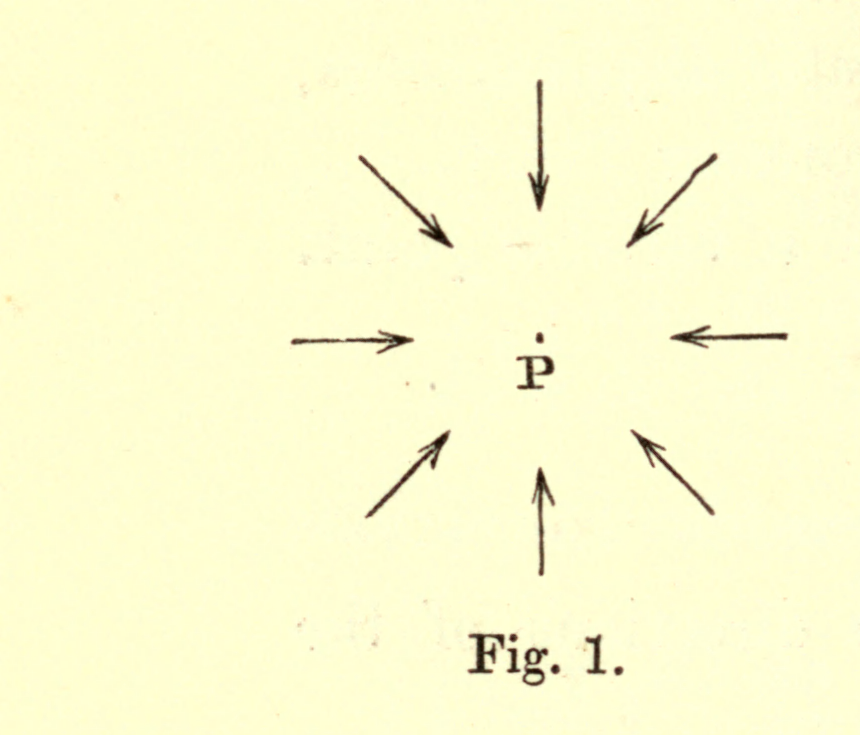
\includegraphics[width=\linewidth]{figures/maxwell_vol1_ia1873_p028_fig1_original_crop.png}
\end{minipage}\hfill
\begin{minipage}[t]{0.68\textwidth}
If we draw a closed surface round \(P\), then, if the surface-integral
of \(\sigma\) over this surface is directed inwards, \(S\nabla\sigma\)
will be positive, and the vector \(\sigma-\sigma_0\) near the point
\(P\) will be on the whole directed towards \(P\), as in the figure
(1). I propose therefore to call the scalar part of \(\nabla\sigma\)
the \textit{convergence} of \(\sigma\) at the point \(P\).
\end{minipage}

\medskip
\noindent
\begin{minipage}[t]{0.28\textwidth}
\centering
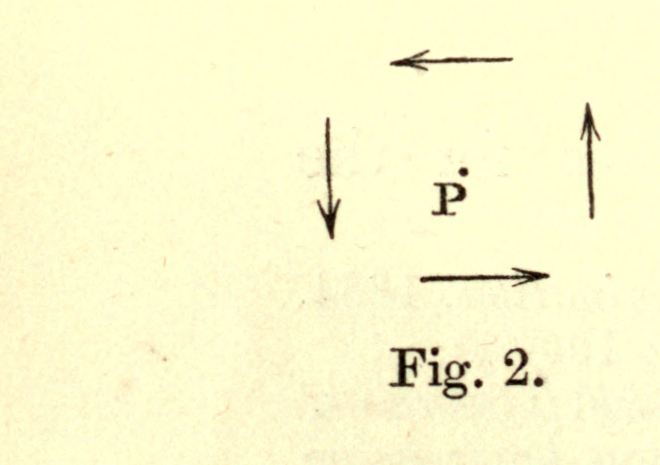
\includegraphics[width=0.92\linewidth]{figures/maxwell_vol1_ia1873_p028_fig2_original_crop.png}
\end{minipage}\hfill
\begin{minipage}[t]{0.68\textwidth}
To interpret the vector part of \(\nabla\sigma\), let us suppose
ourselves to be looking in the direction of the vector whose components
are \(\xi,\eta,\zeta\), and let us examine the vector
\(\sigma-\sigma_0\) near the point \(P\). It will appear as in the
figure (2), this vector being arranged on the whole tangentially in the
direction opposite to the hands of a watch.
\end{minipage}

I propose (with great diffidence) to call the vector part of
\(\nabla\sigma\) the \textit{curl}, or the \textit{version} of
\(\sigma\) at the point \(P\).

\clearpage
\setcounter{footnote}{0}

\noindent
\begin{minipage}[t]{0.62\textwidth}
At Fig. 3 we have an illustration of curl combined with convergence.

Let us now consider the meaning of the equation
\[
V\nabla\sigma=0.
\]
\end{minipage}\hfill
\begin{minipage}[t]{0.26\textwidth}
\centering
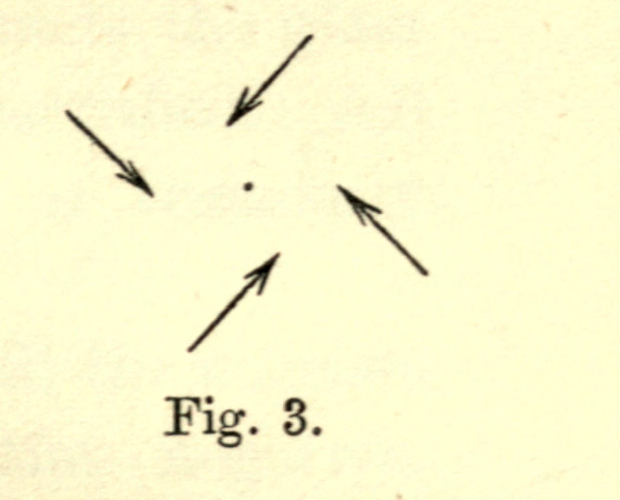
\includegraphics[width=\linewidth]{figures/maxwell_vol1_ia1873_p029_fig3_original_crop.png}
\end{minipage}

\medskip

This implies that \(\nabla\sigma\) is a scalar; or that the vector
\(\sigma\) is the slope of some scalar function \(\Psi\). These
applications of the operator \(\nabla\) are due to Professor
Tait\footnote{\textit{Proceedings R. S. Edin.}, 1862.}. A more complete
development of the theory is given in his paper `On Green's and other
allied Theorems\footnote{\textit{Trans. R. S. Edin.}, 1869--70.},' to
which I refer the reader for the purely Quaternion investigation of the
properties of the operator \(\nabla\).

26.] One of the most remarkable properties of the operator \(\nabla\)
is that when repeated it becomes
\[
\nabla^2=-\left(\frac{d^2}{dx^2}+\frac{d^2}{dy^2}
+\frac{d^2}{dz^2}\right),
\]
an operator occurring in all parts of Physics, which we may refer to as
Laplace's Operator.

This operator is itself essentially scalar. When it acts on a scalar
function the result is scalar, when it acts on a vector function the
result is a vector.

If, with any point \(P\) as centre, we draw a small sphere whose radius
is \(r\), then if \(q_0\) is the value of \(q\) at the centre, and
\(\bar{q}\) the mean value of \(q\) for all points within the sphere,
\[
q_0-\bar{q}=\frac{1}{10}r^2\nabla^2 q;
\]
so that the value at the centre exceeds or falls short of the mean value
according as \(\nabla^2 q\) is positive or negative.

I propose therefore to call \(\nabla^2q\) the \textit{concentration} of
\(q\) at the point \(P\), because it indicates the excess of the value
of \(q\) at that point over its mean value in the neighbourhood of the
point.

If \(q\) is a scalar function, the method of finding its mean value is
well known. If it is a vector function, we must find its mean value by
the rules for integrating vector functions. The result of course is a
vector.

\clearpage
\setcounter{footnote}{0}

\begin{center}
{\Large PART I.}

\vspace{1.4em}

{\Large ELECTROSTATICS.}

\vspace{2.0em}

\rule{0.46\textwidth}{0.4pt}

\vspace{2.0em}

{\Large CHAPTER I.}

\vspace{1.4em}

{\large DESCRIPTION OF PHENOMENA.}

\vspace{1.4em}

\textit{Electrification by Friction.}
\end{center}

27.] \textsc{Experiment I}\footnote{See Sir W. Thomson `On the
Mathematical Theory of Electricity,' \textit{Cambridge and Dublin
Mathematical Journal}, March, 1848.}. Let a piece of glass and a piece
of resin, neither of which exhibits any electrical properties, be rubbed
together and left with the rubbed surfaces in contact. They will still
exhibit no electrical properties. Let them be separated. They will now
attract each other.

If a second piece of glass be rubbed with a second piece of resin, and
if the pieces be then separated and suspended in the neighbourhood of
the former pieces of glass and resin, it may be observed---
\begin{enumerate}
\renewcommand{\labelenumi}{(\arabic{enumi})}
\item That the two pieces of glass repel each other.
\item That each piece of glass attracts each piece of resin.
\item That the two pieces of resin repel each other.
\end{enumerate}

These phenomena of attraction and repulsion are called Electrical
phenomena, and the bodies which exhibit them are said to be
\textit{electrified}, or to be \textit{charged with electricity}.

Bodies may be electrified in many other ways, as well as by friction.

The electrical properties of the two pieces of glass are similar to each
other but opposite to those of the two pieces of resin, the glass
attracts what the resin repels and repels what the resin attracts.

\clearpage
\setcounter{footnote}{0}

If a body electrified in any manner whatever behaves as the glass does,
that is, if it repels the glass and attracts the resin, the body is said
to be \textit{vitreously} electrified, and if it attracts the glass and
repels the resin it is said to be \textit{resinously} electrified. All
electrified bodies are found to be either vitreously or resinously
electrified.

It is the established practice of men of science to call the vitreous
electrification positive, and the resinous electrification negative.
The exactly opposite properties of the two kinds of electrification
justify us in indicating them by opposite signs, but the application of
the positive sign to one rather than to the other kind must be
considered as a matter of arbitrary convention, just as it is a matter
of convention in mathematical diagrams to reckon positive distances
towards the right hand.

No force, either of attraction or of repulsion, can be observed between
an electrified body and a body not electrified. When, in any case,
bodies not previously electrified are observed to be acted on by an
electrified body, it is because they have become \textit{electrified by
induction}.

\begin{center}
\textit{Electrification by Induction.}
\end{center}

28.] \textsc{Experiment II}\footnote{This, and several experiments which
follow, are due to Faraday, `On Static Electrical Inductive Action,'
\textit{Phil. Mag.}, 1843, or \textit{Exp. Res.}, vol. ii. p. 279.}.
Let a hollow vessel of metal be hung up by white silk threads, and let a
similar thread be attached to the lid of the vessel so that the vessel
may be opened or closed without touching it.

Let the pieces of glass and resin be similarly suspended and electrified
as before.

\medskip
\noindent
\begin{minipage}[t]{0.68\textwidth}
Let the vessel be originally unelectrified, then if an electrified piece
of glass is hung up within it by its thread without touching the vessel,
and the lid closed, the outside of the vessel will be found to be
vitreously electrified, and it may be shewn that the electrification
outside of the vessel is exactly the same in whatever part of the
interior space the glass is suspended.

If the glass is now taken out of the vessel without touching it, the
electrification of the glass will be the same as before it was put in,
and that of the vessel will have disappeared.

This electrification of the vessel, which depends on the glass
\end{minipage}\hfill
\begin{minipage}[t]{0.25\textwidth}
\centering
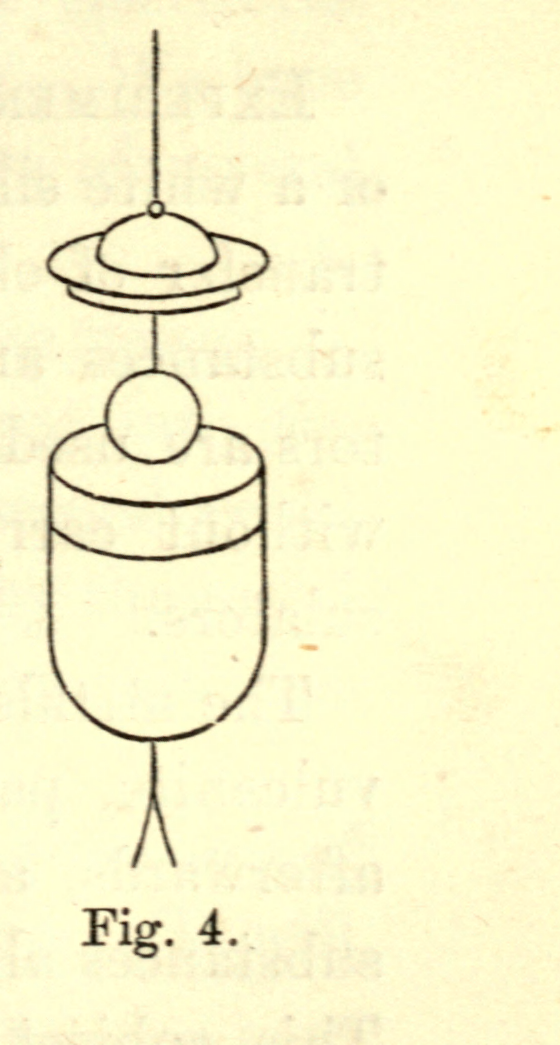
\includegraphics[width=\linewidth]{figures/maxwell_vol1_ia1873_p031_fig4_original_crop.png}
\end{minipage}

\clearpage
\setcounter{footnote}{0}

being within it, and which vanishes when the glass is removed, is
called Electrification by induction.

Similar effects would be produced if the glass were suspended near the
vessel on the outside, but in that \textit{case} we should find an
electrification vitreous in one part of the outside of the vessel and
resinous in another. When the glass is inside the vessel the whole of
the outside is vitreously and the whole of the inside resinously
electrified.

\begin{center}
\textit{Electrification by Conduction.}
\end{center}

29.] \textsc{Experiment III.} Let the metal vessel be electrified by
induction, as in the last experiment, let a second metallic body be
suspended by white silk threads near it, and let a metal wire, similarly
suspended, be brought so as to touch simultaneously the electrified
vessel and the second body.

The second body will now be found to be vitreously electrified, and the
vitreous electrification of the vessel will have diminished.

The electrical condition has been transferred from the vessel to the
second body by means of the wire. The wire is called a
\textit{conductor} of electricity, and the second body is said to be
\textit{electrified by conduction}.

\begin{center}
\textit{Conductors and Insulators.}
\end{center}

\textsc{Experiment IV.} If a glass rod, a stick of resin or
gutta-percha, or a white silk thread, had been used instead of the metal
wire, no transfer of electricity would have taken place. Hence these
latter substances are called Non-conductors of electricity.
Non-conductors are used in electrical experiments to support electrified
bodies without carrying off their electricity. They are then called
Insulators.

The metals are good conductors; air, glass, resins, gutta-percha,
vulcanite, paraffin, \&c. are good insulators; but, as we shall see
afterwards, all substances resist the passage of electricity, and all
substances allow it to pass, though in exceedingly different degrees.
This subject will be considered when we come to treat of the Motion of
electricity. For the present we shall consider only two classes of
bodies, good conductors, and good insulators.

In Experiment II an electrified body produced electrification in the
metal vessel while separated from it by air, a non-conducting medium.
Such a medium, considered as transmitting these electrical effects
without conduction, has been called by Faraday a Dielectric

\clearpage
\setcounter{footnote}{0}

medium, and the action which takes place through it is called
Induction.

In Experiment III the electrified vessel produced electrification in
the second metallic body through the medium of the wire. Let us suppose
the wire removed, and the electrified piece of glass taken out of the
vessel without touching it, and removed to a sufficient distance. The
second body will still exhibit vitreous electrification, but the vessel,
when the glass is removed, will have resinous electrification. If we now
bring the wire into contact with both bodies, conduction will take place
along the wire, and all electrification will disappear from both bodies,
shewing that the electrification of the two bodies was equal and
opposite.

30.] \textsc{Experiment V.} In Experiment II it was shewn that if a
piece of glass, electrified by rubbing it with resin, is hung up in an
insulated metal vessel, the electrification observed outside does not
depend on the position of the glass. If we now introduce the piece of
resin with which the glass was rubbed into the same vessel, without
touching it or the vessel, it will be found that there is no
electrification outside the vessel. From this we conclude that the
electrification of the resin is exactly equal and opposite to that of
the glass. By putting in any number of bodies, electrified in any way,
it may be shewn that the electrification of the outside of the vessel is
that due to the algebraic sum of all the electrifications, those being
reckoned negative which are resinous. We have thus a practical method
of adding the electrical effects of several bodies without altering the
electrification of each.

31.] \textsc{Experiment VI.} Let a second insulated metallic vessel,
\(B\), be provided, and let the electrified piece of glass be put into
the first vessel \(A\), and the electrified piece of resin into the
second vessel \(B\). Let the two vessels be then put in communication by
the metal wire, as in Experiment III. All signs of electrification will
disappear.

Next, let the wire be removed, and let the pieces of glass and of resin
be taken out of the vessels without touching them. It will be found that
\(A\) is electrified resinously and \(B\) vitreously.

If now the glass and the vessel \(A\) be introduced together into a
larger insulated vessel \(C\), it will be found that there is no
electrification outside \(C\). This shews that the electrification of
\(A\) is exactly equal and opposite to that of the piece of glass, and
that of \(B\) may be shewn in the same way to be equal and opposite to
that of the piece of resin.

\clearpage
\setcounter{footnote}{0}

We have thus obtained a method of charging a vessel with a quantity of
electricity exactly equal and opposite to that of an electrified body
without altering the electrification of the latter, and we may in this
way charge any number of vessels with exactly equal quantities of
electricity of either kind, which we may take for provisional units.

32.] \textsc{Experiment VII.} Let the vessel \(B\), charged with a
quantity of positive electricity, which we shall call, for the present,
unity, be introduced into the larger insulated vessel \(C\) without
touching it. It will produce a positive electrification on the outside
of \(C\). Now let \(B\) be made to touch the inside of \(C\). No change
of the external electrification will be observed. If \(B\) is now taken
out of \(C\) without touching it, and removed to a sufficient distance,
it will be found that \(B\) is completely discharged, and that \(C\) has
become charged with a unit of positive electricity.

We have thus a method of transferring the charge of \(B\) to \(C\).

Let \(B\) be now recharged with a unit of electricity, introduced into
\(C\) already charged, made to touch the inside of \(C\), and removed.
It will be found that \(B\) is again completely discharged, so that the
charge of \(C\) is doubled.

If this process is repeated, it will be found that however highly \(C\)
is previously charged, and in whatever way \(B\) is charged, when \(B\)
is first entirely enclosed in \(C\), then made to touch \(C\), and
finally removed without touching \(C\), the charge of \(B\) is
completely transferred to \(C\), and \(B\) is entirely free from
electrification.

This experiment indicates a method of charging a body with any number
of units of electricity. We shall find, when we come to the mathematical
theory of electricity, that the result of this experiment affords an
accurate test of the truth of the theory.

33.] Before we proceed to the investigation of the law of electrical
force, let us enumerate the facts we have already established.

By placing any electrified system inside an insulated hollow conducting
vessel, and examining the resultant effect on the outside of the vessel,
we ascertain the character of the total electrification of the system
placed inside, without any communication of electricity between the
different bodies of the system.

The electrification of the outside of the vessel may be tested with
great delicacy by putting it in communication with an electroscope.

We may suppose the electroscope to consist of a strip of gold-

\clearpage
\setcounter{footnote}{0}

leaf hanging between two bodies charged, one positively, and the other
negatively. If the gold leaf becomes electrified it will incline
towards the body whose electrification is opposite to its own. By
increasing the electrification of the two bodies and the delicacy of
the suspension, an exceedingly small electrification of the gold leaf
may be detected.

When we come to describe electrometers and multipliers we shall find
that there are still more delicate methods of detecting electrification
and of testing the accuracy of our theorems, but at present we shall
suppose the testing to be made by connecting the hollow vessel with a
gold leaf electroscope.

This method was used by Faraday in his very admirable demonstration of
the laws of electrical phenomena\footnote{`On Static Electrical
Inductive Action,' \textit{Phil. Mag.}, 1843, or \textit{Exp. Res.},
vol. ii. p. 249.}.

34.] I. The total electrification of a body, or system of bodies,
remains always the same, except in so far as it receives electrification
from or gives electrification to other bodies.

In all electrical experiments the electrification of bodies is found to
change, but it is always found that this change is due to want of
perfect insulation, and that as the means of insulation are improved,
the loss of electrification becomes less. We may therefore assert that
the electrification of a body placed in a perfectly insulating medium
would remain perfectly constant.

II. When one body electrifies another by conduction, the total
electrification of the two bodies remains the same, that is, the one
loses as much positive or gains as much negative electrification as the
other gains of positive or loses of negative electrification.

For if the two bodies are enclosed in the hollow vessel, no change of
the total electrification is observed.

III. When electrification is produced by friction, or by any other known
method, equal quantities of positive and negative electrification are
produced.

For the electrification of the whole system may be tested in the hollow
vessel, or the process of electrification may be carried on within the
vessel itself, and however intense the electrification of the parts of
the system may be, the electrification of the whole, as indicated by the
gold leaf electroscope, is invariably zero.

The electrification of a body is therefore a physical quantity capable
of measurement, and two or more electrifications can be combined
experimentally with a result of the same kind as when

\clearpage
\setcounter{footnote}{0}

two quantities are added algebraically. We therefore are entitled to use
language fitted to deal with electrification as a quantity as well as a
quality, and to speak of any electrified body as `charged with a certain
quantity of positive or negative electricity'.

35.] While admitting electricity, as we have now done, to the rank of a
physical quantity, we must not too hastily assume that it is, or is not,
a substance, or that it is, or is not, a form of energy, or that it
belongs to any known category of physical quantities. All that we have
hitherto proved is that it cannot be created or annihilated, so that if
the total quantity of electricity within a closed surface is increased
or diminished, the increase or diminution must have passed in or out
through the closed surface.

This is true of matter, and is expressed by the equation known as the
Equation of Continuity in Hydrodynamics.

It is not true of heat, for heat may be increased or diminished within a
closed surface, without passing in or out through the surface, by the
transformation of some other form of energy into heat, or of heat into
some other form of energy.

It is not true even of energy in general if we admit the immediate
action of bodies at a distance. For a body outside the closed surface
may make an exchange of energy with a body within the surface. But if
all apparent action at a distance is the result of the action between
the parts of an intervening medium, and if the nature of this action of
the parts of the medium is clearly understood, then it is conceivable
that in all cases of the increase or diminution of the energy within a
closed surface we may be able to trace the passage of the energy in or
out through that surface.

There is, however, another reason which warrants us in asserting that
electricity, as a physical quantity, synonymous with the total
electrification of a body, is not, like heat, a form of energy. An
electrified system has a certain amount of energy, and this energy can
be calculated by multiplying the quantity of electricity in each of its
parts by another physical quantity, called the Potential of that part,
and taking half the sum of the products. The quantities `Electricity'
and `Potential,' when multiplied together, produce the quantity
`Energy.' It is impossible, therefore, that electricity and energy
should be quantities of the same category, for electricity is only one
of the factors of energy, the other factor being `Potential.'

\clearpage
\setcounter{footnote}{0}

Energy, which is the product of these factors, may also be considered
as the product of several other pairs of factors, such as

\begin{center}
\begin{tabular}{@{}l c p{0.62\textwidth}@{}}
A Force & \(\times\) & A distance through which the force is to act.\\
A Mass & \(\times\) & Gravitation acting through a certain height.\\
A Mass & \(\times\) & Half the square of its velocity.\\
A Pressure & \(\times\) & A volume of fluid introduced into a vessel at that pressure.\\
A Chemical Affinity & \(\times\) & A chemical change, measured by the number of electro-chemical equivalents which enter into combination.
\end{tabular}
\end{center}

If we obtain distinct mechanical ideas of the nature of electric
potential, we may combine these with the idea of energy to determine
the physical category in which `Electricity' is to be placed.

36.] In most theories on the subject, Electricity is treated as a
substance, but inasmuch as there are two kinds of electrification which,
being combined, annul each other, and since we cannot conceive of two
substances annulling each other, a distinction has been drawn between
Free Electricity and Combined Electricity.

\begin{center}
\textit{Theory of Two Fluids.}
\end{center}

In the theory called that of Two Fluids, all bodies, in their
unelectrified state, are supposed to be charged with equal quantities of
positive and negative electricity. These quantities are supposed to be
so great that no process of electrification has ever yet deprived a
body of all the electricity of either kind. The process of
electrification, according to this theory, consists in taking a certain
quantity \(P\) of positive electricity from the body \(A\) and
communicating it to \(B\), or in taking a quantity \(N\) of negative
electricity from \(B\) and communicating it to \(A\), or in some
combination of these processes.

The result will be that \(A\) will have \(P+N\) units of negative
electricity over and above its remaining positive electricity, which is
supposed to be in a state of combination with an equal quantity of
negative electricity. This quantity \(P+N\) is called the Free
electricity, the rest is called the Combined, Latent, or Fixed
electricity.

In most expositions of this theory the two electricities are called
`Fluids,' because they are capable of being transferred from one body to
another, and are, within conducting bodies, extremely

\clearpage
\setcounter{footnote}{0}

mobile. The other properties of fluids, such as their inertia, weight,
and elasticity, are not attributed to them by those who have used the
theory for merely mathematical purposes; but the use of the word Fluid
has been apt to mislead the vulgar, including many men of science who
are not natural philosophers, and who have seized on the word Fluid as
the only term in the statement of the theory which seemed intelligible
to them.

We shall see that the mathematical treatment of the subject has been
greatly developed by writers who express themselves in terms of the
`Two Fluids' theory.. Their results, however, have been deduced
entirely from data which can be proved by experiment, and which must
therefore be true, whether we adopt the theory of two fluids or not. The
experimental verification of the mathematical results therefore is no
evidence for or against the peculiar doctrines of this theory.

The introduction of two fluids permits us to consider the negative
electrification of \(A\) and the positive electrification of \(B\) as
the effect of \textit{any one} of three different processes which would
lead to the same result. We have already supposed it produced by the
transfer of \(P\) units of positive electricity from \(A\) to \(B\),
together with the transfer of \(N\) units of negative electricity from
\(B\) to \(A\). But if \(P+N\) units of positive electricity had been
transferred from \(A\) to \(B\), or if \(P+N\) units of negative
electricity had been transferred from \(B\) to \(A\), the resulting
`free electricity' on \(A\) and on \(B\) would have been the same as
before, but the quantity of `combined electricity' in \(A\) would have
been less in the second case and greater in the third than it was in the
first.

It would appear therefore, according to this theory, that it is possible
to alter not only the amount of free electricity in a body, but the
amount of combined electricity. But no phenomena have ever been observed
in electrified bodies which can be traced to the varying amount of their
combined electricities. Hence either the combined electricities have no
observable properties, or the amount of the combined electricities is
incapable of variation. The first of these alternatives presents no
difficulty to the mere mathematician, who attributes no properties to
the fluids except those of attraction and repulsion, for in this point
of view the two fluids simply annul one another, and their combination
is a true mathematical zero. But to those who cannot use the word Fluid
without thinking of a substance it is difficult to conceive that the
combination of the two fluids shall have no properties at all, so that

\clearpage
\setcounter{footnote}{0}

the addition of more or less of the combination to a body shall not in
any way affect it, either by increasing its mass or its weight, or
altering some of its other properties. Hence it has been supposed by
some, that in every process of electrification exactly equal quantities
of the two fluids are transferred in opposite directions, so that the
total quantity of the two fluids in any body taken together remains
always the same. By this new law they `contrive to save appearances,'
forgetting that there would have been no need of the law except to
reconcile the `two fluids' theory with facts, and to prevent it from
predicting non-existent phenomena.

\begin{center}
\textit{Theory of One Fluid.}
\end{center}

37.] In the theory of One Fluid everything is the same as in the theory
of Two Fluids except that, instead of supposing the two substances equal
and opposite in all respects, one of them, generally the negative one,
has been endowed with the properties and name of Ordinary Matter, while
the other retains the name of The Electric Fluid. The particles of the
fluid are supposed to repel one another according to the law of the
inverse square of the distance, and to attract those of matter according
to the same law. Those of matter are supposed to repel each other and
attract those of electricity. The attraction, however, between units of
the different substances at unit of distance is supposed to be a very
little greater than the repulsion between units of the same kind, so
that a unit of matter combined with a unit of electricity will exert a
force of attraction on a similar combination at a distance, this force,
however, being exceedingly small compared with the force between two
uncombined units.

This residual force is supposed to account for the attraction of
gravitation. Unelectrified bodies are supposed to be charged with as
many units of electricity as they contain of ordinary matter. When they
contain more electricity or less, they are said to be positively or
negatively electrified.

This theory does not, like the Two-Fluid theory, explain too much. It
requires us, however, to suppose the mass of the electric fluid so small
that no attainable positive or negative electrification has yet
perceptibly increased or diminished either the mass or the weight of a
body, and it has not yet been able to assign sufficient reasons why the
vitreous rather than the resinous electrification should be supposed due
to an \textit{excess} of electricity.

One objection has sometimes been urged against this theory by

\clearpage
\setcounter{footnote}{0}

men who ought to have reasoned better. It has been said that the
doctrine that the particles of matter uncombined with electricity
\textit{repel} one another, is in direct antagonism with the
well-established fact that every particle of matter \textit{attracts}
every other particle throughout the universe. If the theory of One Fluid
were true we should have the heavenly bodies repelling one another.

But it is manifest that the heavenly bodies, according to this theory,
if they consisted of matter uncombined with electricity, would be in the
highest state of negative electrification, and would repel each other.
We have no reason to believe that they are in such a highly electrified
state, or could be maintained in that state. The earth and all the
bodies whose attraction has been observed are rather in an unelectrified
state, that is, they contain the normal charge of electricity, and the
only action between them is the residual force lately mentioned. The
artificial manner, however, in which this residual force is introduced
is a much more valid objection to the theory.

In the present treatise I propose, at different stages of the
investigation, to test the different theories in the light of additional
classes of phenomena. For my own part, I look for additional light on
the nature of electricity from a study of what takes place in the space
intervening between the electrified bodies. Such is the essential
character of the mode of investigation pursued by Faraday in his
\textit{Experimental Researches}, and as we go on I intend to exhibit
the results, as developed by Faraday, W. Thomson, \&c., in a connected
and mathematical form, so that we may perceive what phenomena are
explained equally well by all the theories, and what phenomena indicate
the peculiar difficulties of each theory.

\begin{center}
\textit{Measurement of the Force between Electrified Bodies.}
\end{center}

38.] Forces may be measured in various ways. For instance, one of the
bodies may be suspended from one arm of a delicate balance, and weights
suspended from the other arm, till the body, when unelectrified, is in
equilibrium. The other body may then be placed at a known distance
beneath the first, so that the attraction or repulsion of the bodies
when electrified may increase or diminish the apparent weight of the
first. The weight which must be added to or taken from the other arm,
when expressed in dynamical measure, will measure the force between the
bodies. This arrangement was used by Sir W. Snow Harris, and is that
adopted in Sir W. Thomson's absolute electrometers. See Art. 217.

\clearpage
\setcounter{footnote}{0}

It is sometimes more convenient to use a torsion-balance in which a
horizontal arm is suspended by a fine wire or fibre, so as to be capable
of vibrating about the vertical wire as an axis, and the body is attached
to one end of the arm and acted on by the force in the tangential
direction, so as to turn the arm round the vertical axis, and so twist
the suspension wire through a certain angle. The torsional rigidity of
the wire is found by observing the time of oscillation of the arm, the
moment of inertia of the arm being otherwise known, and from the angle
of torsion and the torsional rigidity the force of attraction or
repulsion can be deduced. The torsion-balance was devised by Michell for
the determination of the force of gravitation between small bodies, and
was used by Cavendish for this purpose. Coulomb, working independently
of these philosophers, reinvented it, and successfully applied it to
discover the laws of electric and magnetic forces; and the
torsion-balance has ever since been used in all researches where small
forces have to be measured. See Art. 215.

39.] Let us suppose that by either of these methods we can measure the
force between two electrified bodies. We shall suppose the dimensions of
the bodies small compared with the distance between them, so that the
result may not be much altered by any inequality of distribution of the
electrification on either body, and we shall suppose that both bodies
are so suspended in air as to be at a considerable distance from other
bodies on which they might induce electrification.

It is then found that if the bodies are placed at a fixed distance and
charged respectively with \(e\) and \(e'\) of our provisional units of
electricity, they will repel each other with a force proportional to the
product of \(e\) and \(e'\). If either \(e\) or \(e'\) is negative, that
is, if one of the charges is vitreous and the other resinous, the force
will be attractive, but if both \(e\) and \(e'\) are negative the force
is again repulsive.

We may suppose the first body, \(A\), charged with \(m\) units of
vitreous and \(n\) units of resinous electricity, which may be conceived
separately placed within the body, as in Experiment V.

Let the second body, \(B\), be charged with \(m'\) units of positive and
\(n'\) units of negative electricity.

Then each of the \(m\) positive units in \(A\) will repel each of the
\(m'\) positive units in \(B\) with a certain force, say \(f\), making a
total effect equal to \(m m' f\).

Since the effect of negative electricity is exactly equal and

\clearpage
\setcounter{footnote}{0}

opposite to that of positive electricity, each of the \(m\) positive
units in \(A\) will attract each of the \(n'\) negative units in \(B\)
with the same force \(f\), making a total effect equal to \(m n' f\).

Similarly the \(n\) negative units in \(A\) will attract the \(m'\)
positive units in \(B\) with a force \(n m' f\), and will repel the
\(n'\) negative units in \(B\) with a force \(n n' f\).

The total repulsion will therefore be \((m m' + n n')f\); and the total
attraction will be \((m n' + m' n)f\).

The resultant repulsion will be
\[
  (m m' + n n' - m n' - n m')f
  \quad\hbox{or}\quad
  (m - n)(m' - n')f.
\]
Now \(m - n = e\) is the algebraical value of the charge on \(A\), and
\(m' - n' = e'\) is that of the charge on \(B\), so that the resultant
repulsion may be written \(e e' f\), the quantities \(e\) and \(e'\)
being always understood to be taken with their proper signs.

\begin{center}
\textit{Variation of the Force with the Distance.}
\end{center}

40.] Having established the law of force at a fixed distance, we may
measure the force between bodies charged in a constant manner and placed
at different distances. It is found by direct measurement that the
force, whether of attraction or repulsion, varies inversely as the
square of the distance, so that if \(f\) is the repulsion between two
units at unit distance, the repulsion at distance \(r\) will be
\(f r^{-2}\), and the general expression for the repulsion between
\(e\) units and \(e'\) units at distance \(r\) will be
\[
  f e e' r^{-2}.
\]

\begin{center}
\textit{Definition of the Electrostatic Unit of Electricity.}
\end{center}

41.] We have hitherto used a wholly arbitrary standard for our unit of
electricity, namely, the electrification of a certain piece of glass as
it happened to be electrified at the commencement of our experiments.
We are now able to select a unit on a definite principle, and in order
that this unit may belong to a general system we define it so that \(f\)
may be unity, or in other words---

\begin{quote}
\textit{The electrostatic unit of electricity is that quantity of
electricity which, when placed at unit of distance from an equal
quantity, repels it with unit of force.}
\end{quote}

This unit is called the Electrostatic unit to distinguish it from the
Electromagnetic unit, to be afterwards defined.

We may now write the general law of electrical action in the simple form
\[
  F = e e' r^{-2};\quad \hbox{or,}
\]

\clearpage
\setcounter{footnote}{0}

\begin{quote}
\textit{The repulsion between two small bodies charged respectively with
\(e\) and \(e'\) units of electricity is numerically equal to the
product of the charges divided by the square of the distance.}
\end{quote}

\begin{center}
\textit{Dimensions of the Electrostatic Unit of Quantity.}
\end{center}

42.] If \([Q]\) is the concrete electrostatic unit of quantity itself,
and \(e, e'\) the numerical values of particular quantities; if \([L]\)
is the unit of length, and \(r\) the numerical value of the distance;
and if \([F]\) is the unit of force, and \(F\) the numerical value of
the force, then the equation becomes
\[
  F[F] = e e' r^{-2} [Q^2][L^{-2}];
\]
whence
\[
  [Q] = [L F^{\frac12}]
      = [L^{\frac32} T^{-1} M^{\frac12}].
\]

This unit is called the Electrostatic Unit of electricity. Other units
may be employed for practical purposes, and in other departments of
electrical science, but in the equations of electrostatics quantities
of electricity are understood to be estimated in electrostatic units,
just as in physical astronomy we employ a unit of mass which is founded
on the phenomena of gravitation, and which differs from the units of
mass in common use.

\begin{center}
\textit{Proof of the Law of Electrical Force.}
\end{center}

43.] The experiments of Coulomb with the torsion-balance may be
considered to have established the law of force with a certain
approximation to accuracy. Experiments of this kind, however, are
rendered difficult, and in some degree uncertain, by several disturbing
causes, which must be carefully traced and corrected for.

In the first place, the two electrified bodies must be of sensible
dimensions relative to the distance between them, in order to be capable
of carrying charges sufficient to produce measurable forces. The action
of each body will then produce an effect on the distribution of
electricity on the other, so that the charge cannot be considered as
evenly distributed over the surface, or collected at the centre of
gravity; but its effect must be calculated by an intricate
investigation. This, however, has been done as regards two spheres by
Poisson in an extremely able manner; and the investigation has been
greatly simplified by Sir W. Thomson in his \textit{Theory of Electrical
Images}. See Arts. 172--174.

Another difficulty arises from the action of the electricity induced on
the sides of the case containing the instrument. By

\clearpage
\setcounter{footnote}{0}

making the inside of the instrument accurately cylindric, and making
its inner surface of metal, this effect can be rendered definite and
measurable.

An independent difficulty arises from the imperfect insulation of the
bodies, on account of which the charge continually decreases. Coulomb
investigated the law of dissipation, and made corrections for it in his
experiments.

The methods of insulating charged conductors, and of measuring
electrical effects, have been greatly improved since the time of
Coulomb, particularly by Sir W. Thomson; but the perfect accuracy of
Coulomb's law of force is established, not by any direct experiments
and measurements (which may be used as illustrations of the law), but
by a mathematical consideration of the phenomenon described as
Experiment VII, namely, that an electrified conductor \(B\), if made to
touch the inside of a hollow closed conductor \(C\) and then withdrawn
without touching \(C\), is perfectly discharged, in whatever manner the
outside of \(C\) may be electrified.

By means of delicate electroscopes it is easy to show that no
electricity remains on \(B\) after the operation, and by the
mathematical theory given at Art. 74, this can only be the case if the
force varies inversely as the square of the distance, for if the law
had been of any different form \(B\) would have been electrified.

\begin{center}
\textit{The Electric Field.}
\end{center}

44.] The Electric Field is the portion of space in the neighbourhood of
electrified bodies, considered with reference to electric phenomena. It
may be occupied by air or other bodies, or it may be a so-called
vacuum, from which we have withdrawn every substance which we can act
upon with the means at our disposal.

If an electrified body be placed at any part of the electric field it
will be acted on by a force which will depend, in general, on the shape
of the body and on its charge, if the body is so highly charged as to
produce a sensible disturbance in the previous electrification of the
other bodies.

But if the body is very small and its charge also very small, the
electrification of the other bodies will not be sensibly disturbed, and
we may consider the body as indicating by its centre of gravity a
certain point of the field. The force acting on the body will then be
proportional to its charge, and will be reversed when the charge is
reversed.

\clearpage
\setcounter{footnote}{0}

Let \(e\) be the charge of the body, and \(F\) the force acting on the
body in a certain direction, then when \(e\) is very small \(F\) is
proportional to \(e\), or
\[
  F = R e,
\]
where \(R\) is a quantity depending on the other bodies in the field.
If the charge \(e\) could be made equal to unity without disturbing the
electrification of other bodies we should have \(F=R\).

We shall call \(R\) the Resultant electric force at the given point of
the field.

\begin{center}
\textit{Electric Potential.}
\end{center}

45.] If the small body carrying the small charge \(e\) be moved from the
given point to an indefinite distance from the electrified bodies, it
will experience at each point of its course a force \(R e\), where \(R\)
varies from point to point of the course. Let the whole work done on the
body by these electrical forces be \(V e\), then \(V\) is the potential
at the point of the field from which the body started. If the charge
\(e\) could be made equal to unity without disturbing the electrification
of other bodies, we might define the potential at any point as the work
done on a body charged with unit of electricity in moving from that
point to an infinite distance.

A body electrified positively tends to move from places of greater
positive potential to places of smaller positive, or of negative
potential, and a body negatively electrified tends to move in the
opposite direction.

In a conductor the electrification is distributed exactly as if it were
free to move in the conductor according to the same law. If therefore
two parts of a conductor have different potentials, positive electricity
will move from the part having greater potential to the part having less
potential as long as that difference continues. A conductor therefore
cannot be in electrical equilibrium unless every point in it has the
same potential. This potential is called the Potential of the Conductor.

\begin{center}
\textit{Equipotential Surfaces.}
\end{center}

46.] If a surface described or supposed to be described in the electric
field is such that the electric potential is the same at every point of
the surface it is called an Equipotential surface.

An electrified point constrained to rest upon such a surface will have
no tendency to move from one part of the surface to another, because the
potential is the same at every point. An equipotential surface is
therefore a surface of equilibrium or a level surface.

\clearpage
\setcounter{footnote}{0}

The resultant force at any point of the surface is in the direction of
the normal to the surface, and the magnitude of the force is such that
the work done on an electrical unit in passing from the surface \(V\) to
the surface \(V'\) is \(V-V'\).

No two equipotential surfaces having different potentials can meet one
another, because the same point cannot have more than one potential, but
one equipotential surface may meet itself, and this takes place at all
points and lines of equilibrium.

The surface of a conductor in electrical equilibrium is necessarily an
equipotential surface. If the electrification of the conductor is
positive over the whole surface, then the potential will diminish as we
move away from the surface on every side, and the conductor will be
surrounded by a series of surfaces of lower potential.

But if (owing to the action of external electrified bodies) some regions
of the conductor are electrified positively and others negatively, the
complete equipotential surface will consist of the surface of the
conductor itself together with a system of other surfaces, meeting the
surface of the conductor in the lines which divide the positive from the
negative regions. These lines will be lines of equilibrium, so that an
electrified point placed on one of these lines will experience no force
in any direction.

When the surface of a conductor is electrified positively in some parts
and negatively in others, there must be some other electrified body in
the field besides itself. For if we allow a positively electrified
point, starting from a positively electrified part of the surface, to
move always in the direction of the resultant force upon it, the
potential at the point will continually diminish till the point reaches
either a negatively electrified surface at a potential less than that of
the first conductor, or moves off to an infinite distance. Since the
potential at an infinite distance is zero, the latter case can only
occur when the potential of the conductor is positive.

In the same way a negatively electrified point, moving off from a
negatively electrified part of the surface, must either reach a
positively electrified surface, or pass off to infinity, and the latter
case can only happen when the potential of the conductor is negative.

Therefore, if both positive and negative electrification exists on a
conductor, there must be some other body in the field whose potential
has the same sign as that of the conductor but a greater numerical
value, and if a conductor of any form is alone in the field the
electrification of every part is of the same sign as the potential of
the conductor.

\clearpage
\setcounter{footnote}{0}

\begin{center}
\textit{Lines of Force.}
\end{center}

47.] The line described by a point moving always in the direction of the
resultant force is called a Line of Force. It cuts the equipotential
surfaces at right angles. The properties of lines of force will be more
fully explained afterwards, because Faraday has expressed many of the
laws of electrical action in terms of his conception of lines of force
drawn in the electric field, and indicating both the direction and the
magnitude of the force at every point.

\begin{center}
\textit{Electric Tension.}
\end{center}

48.] Since the surface of a conductor is an equipotential surface, the
resultant force is normal to the surface, and it will be shewn in
Art. 78 that it is proportional to the superficial density of the
electrification. Hence the electricity on any small area of the surface
will be acted on by a force tending \textit{from} the conductor and
proportional to the product of the resultant force and the density, that
is, proportional to the square of the resultant force.

This force which acts outwards as a tension on every part of the
conductor will be called electric Tension. It is measured like ordinary
mechanical tension, by the force exerted on unit of area.

The word Tension has been used by electricians in several vague senses,
and it has been attempted to adopt it in mathematical language as a
synonym for Potential; but on examining the cases in which the word has
been used, I think it will be more consistent with usage and with
mechanical analogy to understand by tension a pulling force of so many
pounds per square inch exerted on the surface of a conductor or
elsewhere. We shall find that the conception of Faraday, that this
electric tension exists not only at the electrified surface but all
along the lines of force, leads to a theory of electric action as a
phenomenon of stress in a medium.

\begin{center}
\textit{Electromotive Force.}
\end{center}

49.] When two conductors at different potentials are connected by a thin
conducting wire, the tendency of electricity to flow along the wire is
measured by the difference of the potentials of the two bodies. The
difference of potentials between two conductors or two points is
therefore called the Electromotive force between them.

Electromotive force may arise from other causes than difference

\clearpage
\setcounter{footnote}{0}

of potential, but these causes are not considered in treating of
statical electricity. We shall consider them when we come to chemical
actions, motions of magnets, inequalities of temperature, \&c.

\begin{center}
\textit{Capacity of a Conductor.}
\end{center}

50.] If one conductor is insulated while all the surrounding conductors
are kept at the zero potential by being put in communication with the
earth, and if the conductor, when charged with a quantity \(E\) of
electricity, has a potential \(V\), the ratio of \(E\) to \(V\) is
called the Capacity of the conductor. If the conductor is completely
enclosed within a conducting vessel without touching it, then the charge
on the inner conductor will be equal and opposite to the charge on the
inner surface of the outer conductor, and will be equal to the capacity
of the inner conductor multiplied by the difference of the potentials of
the two conductors.

\begin{center}
\textit{Electric Accumulators.}
\end{center}

A system consisting of two conductors whose opposed surfaces are
separated from each other by a thin stratum of an insulating medium is
called an electric Accumulator. Its capacity is directly proportional to
the area of the opposed surfaces and inversely proportional to the
thickness of the stratum between them. A Leyden jar is an accumulator in
which glass is the insulating medium. Accumulators are sometimes called
Condensers, but I prefer to restrict the term `condenser' to an
instrument which is used not to hold electricity but to increase its
superficial density.

\begin{center}
\textbf{PROPERTIES OF BODIES IN RELATION TO STATICAL ELECTRICITY.}
\end{center}

\begin{center}
\textit{Resistance to the Passage of Electricity through a Body.}
\end{center}

51.] When a charge of electricity is communicated to any part of a mass
of metal the electricity is rapidly transferred from places of high to
places of low potential till the potential of the whole mass becomes the
same. In the case of pieces of metal used in ordinary experiments this
process is completed in a time too short to be observed, but in the case
of very long and thin wires, such as those used in telegraphs, the
potential does not become uniform till after a sensible time, on account
of the resistance of the wire to the passage of electricity through it.

The resistance to the passage of electricity is exceedingly different in
different substances, as may be seen from the tables at

\clearpage
\setcounter{footnote}{0}

Arts. 362, 366, and 369, which will be explained in treating of
Electric Currents.

All the metals are good conductors, though the resistance of lead is 12
times that of copper or silver, that of iron 6 times, and that of
mercury 60 times that of copper. The resistance of all metals increases
as their temperature rises.

Selenium in its crystalline state may also be regarded as a conductor,
though its resistance is \(3.7 \times 10^{12}\) times that of a piece of
copper of the same dimensions. Its resistance increases as the
temperature rises. Selenium in the amorphous form is a good insulator,
like sulphur.

Many liquids conduct electricity by electrolysis. This mode of
conduction will be considered in Part II. For the present, we may regard
all liquids containing water and all damp bodies as conductors, far
inferior to the metals, but incapable of insulating a charge of
electricity for a sufficient time to be observed.

On the other hand, the gases at the atmospheric pressure, whether dry or
moist, are insulators so nearly perfect when the electric tension is
small that we have as yet obtained no evidence of electricity passing
through them by ordinary conduction. The gradual loss of charge by
electrified bodies may in every case be traced to imperfect insulation
in the supports, the electricity either passing through the substance of
the support or creeping over its surface. Hence, when two charged bodies
are hung up near each other, they will preserve their charges longer if
they are electrified in opposite ways, than if they are electrified in
the same way. For though the electromotive force tending to make the
electricity pass through the air between them is much greater when they
are oppositely electrified, no perceptible loss occurs in this way. The
actual loss takes place through the supports, and the electromotive
force through the supports is greatest when the bodies are electrified
in the same way. The result appears anomalous only when we expect the
loss to occur by the passage of electricity through the air between the
bodies.

Certain kinds of glass when cold are marvellously perfect insulators,
and Sir W. Thomson has preserved charges of electricity for years in
bulbs hermetically sealed. The same glass, however, becomes a conductor
at a temperature below that of boiling water.

Gutta-percha, caoutchouc, vulcanite, paraffin, and resins are good
insulators, the resistance of gutta-percha at \(75^\circ\) F. being
about \(6 \times 10^{19}\) times that of copper.

Ice, crystals, and solidified electrolytes, are also insulators.

\clearpage
\setcounter{footnote}{0}

Certain liquids, such as naphtha, turpentine, and some oils, are
insulators, but inferior to most of the solid insulators.

The resistance of most substances, except the metals, and selenium
and carbon, seems to diminish as the temperature rises.

\begin{center}
\textbf{DIELECTRICS.}
\end{center}

\begin{center}
\textit{Specific Inductive Capacity.}
\end{center}

52.] All bodies whose insulating power is such that when they
are placed between two conductors at different potentials the
electromotive force acting on them does not immediately distribute
their electricity so as to reduce the potential to a constant value, are
called by Faraday Dielectrics.

Faraday discovered that the capacity of an accumulator depends
on the nature of the insulating medium between the two conductors,
as well as on the dimensions and relative position of the conductors
themselves. By substituting other insulating media for air as the
dielectric of the accumulator, without altering it in any other
respect, he found that when air and other gases were employed as
the insulating medium the capacity of the accumulator remained the
same, but that when shell-lac, sulphur, glass, \&c., were substituted
for air, the capacity was increased in a ratio which was different
for each substance.

The ratio of the capacity of an accumulator formed of any dielectric
medium to the capacity of an accumulator of the same form and
dimensions filled with air, was named by Faraday the Specific
Inductive Capacity of the dielectric medium. It is equal to unity
for air and other gases at all pressures, and probably at all
temperatures, and it is greater than unity for all other liquid or solid
dielectrics which have been examined.

If the dielectric is not a good insulator, it is difficult to measure
its inductive capacity, because the accumulator will not hold a
charge for a sufficient time to allow it to be measured; but it is
certain that inductive capacity is a property not confined to good
insulators, and it is probable that it exists in all bodies.

\begin{center}
\textit{Absorption of Electricity.}
\end{center}

53.] It is found that when an accumulator is formed of certain
dielectrics, the following phenomena occur.

When the accumulator has been for some time electrified and is
then suddenly discharged and again insulated, it becomes recharged

\clearpage
\setcounter{footnote}{0}

in the same sense as at first, but to a smaller degree, so that it may
be discharged again several times in succession, these discharges
always diminishing. This phenomenon is called that of the Residual
Discharge.

The instantaneous discharge appears always to be proportional
to the difference of potentials at the instant of discharge, and the
ratio of these quantities is the true capacity of the accumulator;
but if the contact of the discharger is prolonged so as to include
some of the residual discharge, the apparent capacity of the
accumulator, calculated from such a discharge, will be too great.

The accumulator if charged and left insulated appears to lose its
charge by conduction, but it is found that the proportionate rate
of loss is much greater at first than it is afterwards, so that the
measure of conductivity, if deduced from what takes place at first,
would be too great. Thus, when the insulation of a submarine
cable is tested, the insulation appears to improve as the
electrification continues.

Thermal phenomena of a kind at first sight analogous take place
in the case of the conduction of heat when the opposite sides of a
body are kept at different temperatures. In the case of heat we
know that they depend on the heat taken in and given out by the
body itself. Hence, in the case of the electrical phenomena, it
has been supposed that electricity is absorbed and emitted by the
parts of the body. We shall see, however, in Art. 329, that the
phenomena can be explained without the hypothesis of absorption of
electricity, by supposing the dielectric in some degree heterogeneous.

That the phenomenon called Electric Absorption is not an
actual absorption of electricity by the substance may be shewn by
charging the substance in any manner with electricity while it is
surrounded by a closed metallic insulated vessel. If, when the
substance is charged and insulated, the vessel be instantaneously
discharged and then left insulated, no charge is ever communicated
to the vessel by the gradual dissipation of the electrification of the
charged substance within it.

54.] This fact is expressed by the statement of Faraday that
it is impossible to charge matter with an absolute and independent
charge of one kind of electricity\footnote{\textit{Exp. Res.}, vol. i.
series xi. \P\ ii. `On the Absolute Charge of Matter,' and (1244).}.

In fact it appears from the result of every experiment which
has been tried that in whatever way electrical actions may take

\clearpage
\setcounter{footnote}{0}

place among a system of bodies surrounded by a metallic vessel, the
charge on the outside of that vessel is not altered.

Now if any portion of electricity could be forced into a body
so as to be absorbed in it, or to become latent, or in any way
to exist in it, without being connected with an equal portion of
the opposite electricity by lines of induction, or if, after having
being absorbed, it could gradually emerge and return to its
ordinary mode of action, we should find some change of electrification
in the surrounding vessel.

As this is never found to be the case, Faraday concluded that
it is impossible to communicate an absolute charge to matter, and
that no portion of matter can by any change of state evolve or
render latent one kind of electricity or the other. He therefore
regarded induction as `the essential function both in the first
development and the consequent phenomena of electricity.' His
`induction' is (1298) a polarized state of the particles of the
dielectric, each particle being positive on one side and negative
on the other, the positive and the negative electrification of each
particle being always exactly equal.

\begin{center}
\textit{Disruptive Discharge\footnote{See Faraday, \textit{Exp. Res.}, vol. i.,
series xii. and xiii.}.}
\end{center}

55.] If the electromotive force acting at any point of a dielectric
is gradually increased, a limit is at length reached at which there
is a sudden electrical discharge through the dielectric, generally
accompanied with light and sound, and with a temporary or
permanent rupture of the dielectric.

The intensity of the electromotive force when this takes place
depends on the nature of the dielectric. It is greater, for instance,
in dense air than in rare air, and greater in glass than in air, but
in every case, if the electromotive force be made great enough,
the dielectric gives way and its insulating power is destroyed, so
that a current of electricity takes place through it. It is for this
reason that distributions of electricity for which the electric resultant
force becomes anywhere infinite cannot exist in nature.

\begin{center}
\textit{The Electric Glow.}
\end{center}

Thus, when a conductor having a sharp point is electrified,
the theory, based on the hypothesis that it retains its charge,
leads to the conclusion that as we approach the point the superficial
density of the electricity increases without limit, so that at
the point itself the surface-density, and therefore the resultant

\clearpage
\setcounter{footnote}{0}

electrical force, would be infinite. If the air, or other surrounding
dielectric, had an invincible insulating power, this result would
actually occur; but the fact is, that as soon as the resultant force
in the neighbourhood of the point has reached a certain limit, the
insulating power of the air gives way, so that the air close to
the point becomes a conductor. At a certain distance from the
point the resultant force is not sufficient to break through the
insulation of the air, so that the electric current is checked, and
the electricity accumulates in the air round the point.

The point is thus surrounded by particles of air charged with
electricity of the same kind with its own. The effect of this charged
air round the point is to relieve the air at the point itself from
part of the enormous electromotive force which it would have
experienced if the conductor alone had been electrified. In fact the
surface of the electrified body is no longer pointed, because the
point is enveloped by a rounded mass of electrified air, the surface
of which, rather than that of the solid conductor, may be regarded
as the outer electrified surface.

If this portion of electrified air could be kept still, the
electrified body would retain its charge, if not on itself at least in its
neighbourhood, but the charged particles of air being free to move
under the action of electrical force, tend to move away from the
electrified body because it is charged with the same kind of electricity.
The charged particles of air therefore tend to move off in the
direction of the lines of force and to approach those surrounding bodies
which are oppositely electrified. When they are gone, other
uncharged particles take their place round the point, and since these
cannot shield those next the point itself from the excessive electric
tension, a new discharge takes place, after which the newly
charged particles move off, and so on as long as the body remains
electrified.

In this way the following phenomena are produced:---At and
close to the point there is a steady glow, arising from the constant
discharges which are taking place between the point and the
air very near it.

The charged particles of air tend to move off in the same general
direction, and thus produce a current of air from the point,
consisting of the charged particles, and probably of others carried along
by them. By artificially aiding this current we may increase the
glow, and by checking the formation of the current we may
prevent the continuance of the glow.

\clearpage
\setcounter{footnote}{0}

The electric wind in the neighbourhood of the point is sometimes
very rapid, but it soon loses its velocity, and the air with its charged
particles is carried about with the general motions of the atmosphere,
and constitutes an invisible electric cloud. When the charged
particles come near to any conducting surface, such as a wall, they
induce on that surface an electrification opposite to their own, and
are then attracted towards the wall, but since the electromotive
force is small they may remain for a long time near the wall
without being drawn up to the surface and discharged. They
thus form an electrified atmosphere clinging to conductors, the
presence of which may sometimes be detected by the electrometer.

The electrical forces, however, acting between charged portions
of air and other bodies are exceedingly feeble compared with the
forces which produce winds arising from inequalities of density
due to differences of temperature, so that it is very improbable
that any observable part of the motion of ordinary thunder clouds
arises from electrical causes.

The passage of electricity from one place to another by the
motion of charged particles is called Electrical Convection or
Convective Discharge.

The electrical glow is therefore produced by the constant passage
of electricity through a small portion of air in which the tension
is very high, so as to charge the surrounding particles of air which
are continually swept off by the electric wind, which is an essential
part of the phenomenon.

The glow is more easily formed in rare air than in dense air,
and more easily when the point is positive than when it is negative.
This and many other differences between positive and negative
electrification must be studied by those who desire to discover
something about the nature of electricity. They have not, however,
been satisfactorily brought to bear upon any existing theory.

\begin{center}
\textit{The Electric Brush.}
\end{center}

56.] The electric brush is a phenomenon which may be produced
by electrifying a blunt point or small ball so as to produce
an electric field in which the tension diminishes, but in a less rapid
manner, as we leave the surface. It consists of a succession of
discharges, ramifying as they diverge from the ball into the air,
and terminating either by charging portions of air or by reaching
some other conductor. It is accompanied by a sound, the pitch of
which depends on the interval between the successive discharges,
and there is no current of air as in the case of the glow.

\clearpage
\setcounter{footnote}{0}

\begin{center}
\textit{The Electric Spark.}
\end{center}

57.] When the tension in the space between two conductors is
considerable all the way between them, as in the case of two balls
whose distance is not great compared with their radii, the discharge,
when it occurs, usually takes the form of a spark, by which nearly
the whole electrification is discharged at once.

In this case, when any part of the dielectric has given way,
the parts on either side of it in the direction of the electric force
are put into a state of greater tension so that they also give way,
and so the discharge proceeds right through the dielectric, just as
when a little rent is made in the edge of a piece of paper a tension
applied to the paper in the direction of the edge causes the paper to
be torn through, beginning at the rent, but diverging occasionally
where there are weak places in the paper. The electric spark in
the same way begins at the point where the electric tension first
overcomes the insulation of the dielectric, and proceeds from that
point, in an apparently irregular path, so as to take in other weak
points, such as particles of dust floating in air.

\begin{center}
\textit{On the Electric Force required to produce a Spark in Air.}
\end{center}

In the experiments of Sir W. Thomson\footnote{\textit{Proc. R. S.}, 1860;
or, Reprint, chap. xix.} the electromotive force
required to produce a spark across strata of air of various thicknesses
was measured by means of an electrometer.

The sparks were made to pass between two surfaces, one of which
was plane, and the other only sufficiently convex to make the sparks
occur always at the same place.

The difference of potential required to cause a spark to pass was
found to increase with the distance, but in a less rapid ratio, so that
the electric force at any point between the surfaces, which is the
quotient of the difference of potential divided by the distance, can
be raised to a greater value without a discharge when the stratum
of air is thin.

When the stratum of air is very thin, say .00254 of a centimètre,
the resultant force required to produce a spark was found to be
527.7, in terms of centimètres and grammes. This corresponds to
an electric tension of 11.29 grammes weight per square centimètre.

When the distance between the surfaces is about a millimètre
the electric force is about 130, and the electric tension .68 grammes
weight per square centimètre. It is probable that the value for

\clearpage
\setcounter{footnote}{0}

greater distances is not much less than this. The ordinary pressure
of the atmosphere is about 1032 grammes per square centimètre.

It is difficult to explain why a thin stratum of air should require
a greater force to produce a disruptive discharge across it than a
thicker stratum. Is it possible that the air very near to the surface
of dense bodies is condensed, so as to become a better insulator?
or does the potential of an electrified conductor differ from
that of the air in contact with it by a quantity having a maximum
value just before discharge, so that the observed difference of
potential of the conductors is in every case greater than the
difference of potentials on the two sides of the stratum of air by a
constant quantity equivalent to the addition of about .005 of an
inch to the thickness of the stratum? See Art. 370.

All these phenomena differ considerably in different gases, and in
the same gas at different densities. Some of the forms of electrical
discharge through rare gases are exceedingly remarkable. In some
cases there is a regular alternation of luminous and dark strata, so
that if the electricity, for example, is passing along a tube containing
a very small quantity of gas, a number of luminous disks will
be seen arranged transversely at nearly equal intervals along the
axis of the tube and separated by dark strata. If the strength of
the current be increased a new disk will start into existence, and
it and the old disks will arrange themselves in closer order. In
a tube described by Mr. Gassiot\footnote{\textit{Intellectual Observer}, March, 1866.}
the light of each of the disks
is bluish on the negative and reddish on the positive side, and
bright red in the central stratum.

These, and many other phenomena of electrical discharge, are
exceedingly important, and when they are better understood they
will probably throw great light on the nature of electricity as well
as on the nature of gases and of the medium pervading space. At
present, however, they must be considered as outside the domain of
the mathematical theory of electricity.

\begin{center}
\textit{Electric Phenomena of Tourmaline.}
\end{center}

58.] Certain crystals of tourmaline, and of other minerals, possess
what may be called Electric Polarity. Suppose a crystal of
tourmaline to be at a uniform temperature, and apparently free from
electrification on its surface. Let its temperature be now raised,
the crystal remaining insulated. One end will be found positively

\clearpage
\setcounter{footnote}{0}

and the other end negatively electrified. Let the surface be deprived
of this apparent electrification by means of a flame or otherwise,
then if the crystal be made still hotter, electrification of the
same kind as before will appear, but if the crystal be cooled the
end which was positive when the crystal was heated will become
negative.

These electrifications are observed at the extremities of the
crystallographic axis. Some crystals are terminated by a six-sided
pyramid at one end and by a three-sided pyramid at the other.
In these the end having the six-sided pyramid becomes positive
when the crystal is heated.

Sir W. Thomson supposes every portion of these and other
hemihedral crystals to have a definite electric polarity, the intensity
of which depends on the temperature. When the surface is passed
through a flame, every part of the surface becomes electrified to
such an extent as to exactly neutralize, for all external points,
the effect of the internal polarity. The crystal then has no
external electrical action, nor any tendency to change its mode of
electrification. But if it be heated or cooled the interior polarization
of each particle of the crystal is altered, and can no longer
be balanced by the superficial electrification, so that there is a
resultant external action.

\begin{center}
\textit{Plan of this Treatise.}
\end{center}

59.] In the following treatise I propose first to explain the ordinary
theory of electrical action, which considers it as depending only
on the electrified bodies and on their relative position, without
taking account of any phenomena which may take place in the
surrounding media. In this way we shall establish the law of the
inverse square, the theory of the potential, and the equations of
Laplace and Poisson. We shall next consider the charges and
potentials of a system of electrified conductors as connected by
a system of equations, the coefficients of which may be supposed
to be determined by experiment in those cases in which our present
mathematical methods are not applicable, and from these we shall
determine the mechanical forces acting between the different
electrified bodies.

We shall then investigate certain general theorems by which
Green, Gauss, and Thomson have indicated the conditions of
solution of problems in the distribution of electricity. One result
of these theorems is, that if Poisson's equation is satisfied by any

\clearpage
\setcounter{footnote}{0}

function, and if at the surface of every conductor the function
has the value of the potential of that conductor, then the function
expresses the actual potential of the system at every point. We
also deduce a method of finding problems capable of exact solution.

In Thomson's theorem, the total energy of the system is expressed
in the form of the integral of a certain quantity extended over
the whole space between the electrified bodies, and also in the form
of an integral extended over the electrified surfaces only. The
equation between these two expressions may be thus interpreted
physically. We may conceive the relation into which the electrified
bodies are thrown, either as the result of the state of the intervening
medium, or as the result of a direct action between the electrified
bodies at a distance. If we adopt the latter conception, we may
determine the law of the action, but we can go no further in
speculating on its cause. If, on the other hand, we adopt the
conception of action through a medium, we are led to enquire into
the nature of that action in each part of the medium.

It appears from the theorem, that if we are to look for the seat
of the electric energy in the different parts of the dielectric medium,
the amount of energy in any small part must depend on the square
of the intensity of the resultant electromotive force at that place
multiplied by a coefficient called the specific inductive capacity
of the medium.

It is better, however, in considering the theory of dielectrics in
the most general point of view, to distinguish between the electromotive
force at any point and the electric polarization of the medium at
that point, since these directed quantities, though related to one
another, are not, in some solid substances, in the same direction.
The most general expression for the electric energy of the medium
per unit of volume is half the product of the electromotive force
and the electric polarization multiplied by the cosine of the angle
between their directions.

In all fluid dielectrics the electromotive force and the electric
polarization are in the same direction and in a constant ratio.
If we calculate on this hypothesis the total energy residing in
the medium, we shall find it equal to the energy due to the
electrification of the conductors on the hypothesis of direct action
at a distance. Hence the two hypotheses are mathematically equivalent.

If we now proceed to investigate the mechanical state of the
medium on the hypothesis that the mechanical action observed

\clearpage
\setcounter{footnote}{0}

between electrified bodies is exerted through and by means of
the medium, as in the familiar instances of the action of one body
on another by means of the tension of a rope or the pressure of
a rod, we find that the medium must be in a state of mechanical
stress.

The nature of this stress is, as Faraday pointed out\footnote{\textit{Exp. Res.}, series xi. 1297.},
a tension along the lines of force combined with an equal pressure
in all directions at right angles to these lines. The magnitude of
these stresses is proportional to the energy of the electrification,
or, in other words, to the square of the resultant electromotive
force multiplied by the specific inductive capacity of the medium.

This distribution of stress is the only one consistent with the
observed mechanical action on the electrified bodies, and also with
the observed equilibrium of the fluid dielectric which surrounds
them. I have therefore thought it a warrantable step in scientific
procedure to assume the actual existence of this state of stress,
and to follow the assumption into its consequences. Finding the
phrase \textit{electric tension} used in several vague senses, I have
attempted to confine it to what I conceive to have been in the mind
of some of those who have used it, namely, the state of stress in
the dielectric medium which causes motion of the electrified bodies,
and leads, when continually augmented, to disruptive discharge.
Electric tension, in this sense, is a tension of exactly the same
kind, and measured in the same way, as the tension of a rope,
and the dielectric medium, which can support a certain tension
and no more, may be said to have a certain strength in exactly
the same sense as the rope is said to have a certain strength.
Thus, for example, Thomson has found that air at the ordinary
pressure and temperature can support an electric tension of 9600
grains weight per square foot before a spark passes.

60.] From the hypothesis that electric action is not a direct
action between bodies at a distance, but is exerted by means of
the medium between the bodies, we have deduced that this medium
must be in a state of stress. We have also ascertained the character
of the stress, and compared it with the stresses which may occur
in solid bodies. Along the lines of force there is tension, and
perpendicular to them there is pressure, the numerical magnitude
of these forces being equal, and each proportional to the square
of the resultant force at the point. Having established these
results, we are prepared to take another step, and to form


an idea of the nature of the electric polarization of the dielectric
medium.

An elementary portion of a body may be said to be polarized
when it acquires equal and opposite properties on two opposite
sides. The idea of internal polarity may be studied to the greatest
advantage as exemplified in permanent magnets, and it will be
explained at greater length when we come to treat of magnetism.

The electric polarization of an elementary portion of a dielectric
is a forced state into which the medium is thrown by the action
of electromotive force, and which disappears when that force is
removed. We may conceive it to consist in what we may call
an electrical displacement, produced by the electromotive force.
When the electromotive force acts on a conducting medium it
produces a current through it, but if the medium is a non-conductor
or dielectric, the current cannot flow through the medium, but the
electricity is displaced within the medium in the direction of the
electromotive force, the extent of this displacement depending on
the magnitude of the electromotive force, so that if the electromotive
force increases or diminishes the electric displacement increases
and diminishes in the same ratio.

The amount of the displacement is measured by the quantity of
electricity which crosses unit of area, while the displacement increases
from zero to its actual amount. This, therefore, is the measure of
the electric polarization.

The analogy between the action of electromotive force in producing
electric displacement and of ordinary mechanical force in producing
the displacement of an elastic body is so obvious that I have ventured
to call the ratio of the electromotive force to the corresponding
electric displacement the \textit{coefficient of electric elasticity} of the
medium. This coefficient is different in different media, and varies
inversely as the specific inductive capacity of each medium.

The variations of electric displacement evidently constitute electric
currents. These currents, however, can only exist during the
variation of the displacement, and therefore, since the displacement
cannot exceed a certain value without causing disruptive discharge,
they cannot be continued indefinitely in the same direction, like the
currents through conductors.

In tourmaline, and other pyro-electric crystals, it is probable that
a state of electric polarization exists, which depends upon temperature,
and does not require an external electromotive force to produce it.
If the interior of a body were in a state of permanent

\clearpage
\setcounter{footnote}{0}

electric polarization, the outside would gradually become charged
in such a manner as to neutralize the action of the internal electrification
for all points outside the body. This external superficial charge could
not be detected by any of the ordinary tests, and could not be removed
by any of the ordinary methods for discharging superficial electrification.
The internal polarization of the substance would therefore never be
discovered unless by some means, such as change of temperature, the
amount of the internal polarization could be increased or diminished.
The external electrification would then be no longer capable of
neutralizing the external effect of the internal polarization, and an
apparent electrification would be observed, as in the case of tourmaline.

If a charge \(e\) is uniformly distributed over the surface of a sphere,
the resultant force at any point of the medium surrounding the sphere
is numerically equal to the charge \(e\) divided by the square of the
distance from the centre of the sphere. This resultant force, according
to our theory, is accompanied by a displacement of electricity in a
direction outwards from the sphere.

If we now draw a concentric spherical surface of radius \(r\), the
whole displacement, \(E\), through this surface will be proportional to
the resultant force multiplied by the area of the spherical surface.
But the resultant force is directly as the charge \(e\) and inversely as
the square of the radius, while the area of the surface is directly as
the square of the radius.

Hence the whole displacement, \(E\), is proportional to the charge
\(e\), and is independent of the radius.

To determine the ratio between the charge \(e\), and the quantity of
electricity, \(E\), displaced outwards through the spherical surface, let
us consider the work done upon the medium in the region between two
concentric spherical surfaces, while the displacement is increased from
\(E\) to \(E+\delta E\). If \(V_1\) and \(V_2\) denote the potentials at
the inner and the outer of these surfaces respectively, the electromotive
force by which the additional displacement is produced is \(V_1-V_2\),
so that the work spent in augmenting the displacement is
\((V_1-V_2)\delta E\).

If we now make the inner surface coincide with that of the electrified
sphere, and make the radius of the other infinite, \(V_1\) becomes
\(V\), the potential of the sphere, and \(V_2\) becomes zero, so that the
whole work done in the surrounding medium is \(V\delta E\).

But by the ordinary theory, the work done in augmenting the charge
is \(V\delta e\), and if this is spent, as we suppose, in augmenting

\clearpage
\setcounter{footnote}{0}

the displacement, \(\delta E=\delta e\), and since \(E\) and \(e\) vanish
together, \(E=e\), or---\textit{The displacement outwards through any
spherical surface concentric with the sphere is equal to the charge on
the sphere.}

To fix our ideas of electric displacement, let us consider an accumulator
formed of two conducting plates \(A\) and \(B\), separated by a stratum
of a dielectric \(C\). Let \(W\) be a conducting wire joining \(A\) and
\(B\), and let us suppose that by the action of an electromotive force
a quantity \(Q\) of positive electricity is transferred along the wire
from \(B\) to \(A\). The positive electrification of \(A\) and the negative
electrification of \(B\) will produce a certain electromotive force
acting from \(A\) towards \(B\) in the dielectric stratum, and this will
produce an electric displacement from \(A\) towards \(B\) within the
dielectric. The amount of this displacement, as measured by the
quantity of electricity forced across an imaginary section of the
dielectric dividing it into two strata, will be, according to our theory,
exactly \(Q\). See Arts. 75, 76, 111.

It appears, therefore, that at the same time that a quantity \(Q\) of
electricity is being transferred along the wire by the electromotive
force from \(B\) towards \(A\), so as to cross every section of the wire,
the same quantity of electricity crosses every section of the dielectric
from \(A\) towards \(B\) by reason of the electric displacement.

The reverse motions of electricity will take place during the discharge
of the accumulator. In the wire the discharge will be \(Q\) from \(A\)
to \(B\), and in the dielectric the displacement will subside, and a
quantity of electricity \(Q\) will cross every section from \(B\) towards
\(A\).

Every case of electrification or discharge may therefore be considered
as a motion in a closed circuit, such that at every section of the
circuit the same quantity of electricity crosses in the same time, and
this is the case, not only in the voltaic circuit where it has always
been recognised, but in those cases in which electricity has been
generally supposed to be accumulated in certain places.

61.] We are thus led to a very remarkable consequence of the theory
which we are examining, namely, that the motions of electricity are
like those of an \textit{incompressible fluid}, so that the total quantity
within an imaginary fixed closed surface remains always the same.
This result appears at first sight in direct contradiction to the fact
that we can charge a conductor and then introduce

\clearpage
\setcounter{footnote}{0}

it into the closed space, and so alter the quantity of electricity within
that space. But we must remember that the ordinary theory takes no
account of the electric displacement in the substance of dielectrics
which we have been investigating, but confines its attention to the
electrification at the bounding surfaces of the conductors and
dielectrics. In the case of the charged conductor let us suppose the
charge to be positive, then if the surrounding dielectric extends on all
sides beyond the closed surface there will be electric polarization,
accompanied with displacement from within outwards all over the closed
surface, and the surface-integral of the displacement taken over the
surface will be equal to the charge on the conductor within.

Thus when the charged conductor is introduced into the closed space
there is immediately a displacement of a quantity of electricity equal
to the charge through the surface from within outwards, and the whole
quantity within the surface remains the same.

The theory of electric polarization will be discussed at greater length
in Chapter V, and a mechanical illustration of it will be given in
Art. 334, but its importance cannot be fully understood till we arrive
at the study of electromagnetic phenomena.

62.] The peculiar features of the theory as we have now developed
them are:---

That the energy of electrification resides in the dielectric medium,
whether that medium be solid, liquid, or gaseous, dense or rare, or
even deprived of ordinary gross matter, provided it be still capable of
transmitting electrical action.

That the energy in any part of the medium is stored up in the form
of a state of constraint called electric polarization, the amount of
which depends on the resultant electromotive force at the place.

That electromotive force acting on a dielectric produces what we have
called electric displacement, the relation between the force and the
displacement being in the most general case of a kind to be afterwards
investigated in treating of conduction, but in the most important cases
the force is in the same direction as the displacement, and is numerically
equal to the displacement multiplied by a quantity which we have called
the coefficient of electric elasticity of the dielectric.

That the energy per unit of volume of the dielectric arising from the
electric polarization is half the product of the electromotive

\clearpage
\setcounter{footnote}{0}

force and the electric displacement multiplied, if necessary, by the
cosine of the angle between their directions.

That in fluid dielectrics the electric polarization is accompanied by
a tension in the direction of the lines of force combined with an equal
pressure in all directions at right angles to the lines of force, the
amount of the tension or pressure per unit of area being numerically
equal to the energy per unit of volume at the same place.

That the surfaces of any elementary portion into which we may conceive
the volume of the dielectric divided must be conceived to be electrified,
so that the surface-density at any point of the surface is equal in
magnitude to the displacement through that point of the surface
\textit{reckoned inwards}, so that if the displacement is in the positive
direction, the surface of the element will be electrified negatively on
the positive side and positively on the negative side. These superficial
electrifications will in general destroy one another when consecutive
elements are considered, except where the dielectric has an internal
charge, or at the surface of the dielectric.

That whatever electricity may be, and whatever we may understand by
the movement of electricity, the phenomenon which we have called electric
displacement is a movement of electricity in the same sense as the
transference of a definite quantity of electricity through a wire is a
movement of electricity, the only difference being that in the dielectric
there is a force which we have called electric elasticity which acts
against the electric displacement, and forces the electricity back when
the electromotive force is removed; whereas in the conducting wire the
electric elasticity is continually giving way, so that a current of true
conduction is set up, and the resistance depends, not on the total
quantity of electricity displaced from its position of equilibrium, but
on the quantity which crosses a section of the conductor in a given
time.

That in every case the motion of electricity is subject to the same
condition as that of an incompressible fluid, namely, that at every
instant as much must flow out of any given closed space as flows into it.

It follows from this that every electric current must form a closed
circuit. The importance of this result will be seen when we investigate
the laws of electro-magnetism.

Since, as we have seen, the theory of direct action at a distance is
mathematically identical with that of action by means of a

\clearpage
\setcounter{footnote}{0}

medium, the actual phenomena may be explained by the one theory as
well as by the other, provided suitable hypotheses be introduced when
any difficulty occurs. Thus, Mossotti has deduced the mathematical
theory of dielectrics from the ordinary theory of attraction by merely
giving an electric instead of a magnetic interpretation to the symbols
in the investigation by which Poisson has deduced the theory of magnetic
induction from the theory of magnetic fluids. He assumes the existence
within the dielectric of small conducting elements, capable of having
their opposite surfaces oppositely electrified by induction, but not
capable of losing or gaining electricity on the whole, owing to their
being insulated from each other by a non-conducting medium. This theory
of dielectrics is consistent with the laws of electricity, and may be
actually true. If it is true, the specific inductive capacity of a
dielectric may be greater, but cannot be less, than that of air or
vacuum. No instance has yet been found of a dielectric having an
inductive capacity less than that of air, but if such should be
discovered, Mossotti's theory must be abandoned, although his formulae
would all remain exact, and would only require us to alter the sign of
a coefficient.

In the theory which I propose to develope, the mathematical methods
are founded upon the smallest possible amount of hypothesis, and thus
equations of the same form are found applicable to phenomena which are
certainly of quite different natures, as, for instance, electric induction
through dielectrics; conduction through conductors, and magnetic
induction. In all these cases the relation between the force and the
effect produced is expressed by a set of equations of the same kind,
so that when a problem in one of these subjects is solved, the problem
and its solution may be translated into the language of the other
subjects and the results in their new form will also be true.

\clearpage
\setcounter{footnote}{0}

\section*{CHAPTER II.}

\section*{ELEMENTARY MATHEMATICAL THEORY OF STATICAL ELECTRICITY.}

\begin{center}
\textit{Definition of Electricity as a Mathematical Quantity.}
\end{center}

63.] We have seen that the actions of electrified bodies are such that
the electrification of one body may be equal to that of another, or to
the sum of the electrifications of two bodies, and that when two bodies
are equally and oppositely electrified they have no electrical effect on
external bodies when placed together within a closed insulated conducting
vessel. We may express all these results in a concise and consistent
manner by describing an electrified body as \textit{charged with a certain
quantity of electricity}, which we may denote by \(e\). When the
electrification is positive, that is, according to the usual convention,
vitreous, \(e\) will be a positive quantity. When the electrification
is negative or resinous, \(e\) will be negative, and the quantity \(-e\)
may be interpreted either as a negative quantity of vitreous electricity
or as a positive quantity of resinous electricity.

The effect of adding together two equal and opposite charges of
electricity, \(+e\) and \(-e\), is to produce a state of no electrification
expressed by zero. We may therefore regard a body not electrified as
virtually charged with equal and opposite charges of indefinite
magnitude, and an electrified body as virtually charged with unequal
quantities of positive and negative electricity, the algebraic sum of
these charges constituting the observed electrification. It is manifest,
however, that this way of regarding an electrified body is entirely
artificial, and may be compared to the conception of the velocity of a
body as compounded of two or more different velocities, no one of which
is the actual velocity of the body. When we speak therefore of a body
being charged with a quantity \(e\) of electricity we mean simply that
the body is electrified, and that the electrification is vitreous or
resinous according as \(e\) is positive or negative.

\clearpage
\setcounter{footnote}{0}

\begin{center}
ON ELECTRIC DENSITY.
\end{center}

\begin{center}
\textit{Distribution in Three Dimensions.}
\end{center}

64.] \textit{Definition.} The electric volume-density at a given point in
space is the limiting ratio of the quantity of electricity within a
sphere whose centre is the given point to the volume of the sphere,
when its radius is diminished without limit.

We shall denote this ratio by the symbol \(\rho\), which may be positive
or negative.

\begin{center}
\textit{Distribution on a Surface.}
\end{center}

It is a result alike of theory and of experiment, that, in certain cases,
the electrification of a body is entirely on the surface. The density
at a point on the surface, if defined according to the method given
above, would be infinite. We therefore adopt a different method for
the measurement of surface-density.

\textit{Definition.} The electric density at a given point on a surface is
the limiting ratio of the quantity of electricity within a sphere whose
centre is the given point to the area of the surface contained within
the sphere, when its radius is diminished without limit.

We shall denote the surface-density by the symbol \(\sigma\).

Those writers who supposed electricity to be a material fluid or a
collection of particles, were obliged in this case to suppose the
electricity distributed on the surface in the form of a stratum of a
certain thickness \(\theta\), its density being \(\rho_0\), or that value of
\(\rho\) which would result from the particles having the closest contact
of which they are capable. It is manifest that on this theory
\[
\rho_0\theta=\sigma.
\]

When \(\sigma\) is negative, according to this theory, a certain stratum
of thickness \(\theta\) is left entirely devoid of positive electricity, and
filled entirely with negative electricity.

There is, however, no experimental evidence either of the electric
stratum having any thickness, or of electricity being a fluid or a
collection of particles. We therefore prefer to do without the symbol
for the thickness of the stratum, and to use a special symbol for
surface-density.

\begin{center}
\textit{Distribution along a Line.}
\end{center}

It is sometimes convenient to suppose electricity distributed on a line,
that is, a long narrow body of which we neglect the

\clearpage
\setcounter{footnote}{0}

thickness. In this case we may define the line-density at any point
to be the limiting ratio of the electricity on an element of the line
to the length of that element when the element is diminished without
limit.

If \(\lambda\) denotes the line-density, then the whole quantity of
electricity on a curve is
\[
e=\int \lambda\,ds,
\]
where \(ds\) is the element of the curve.

Similarly, if \(\sigma\) is the surface-density, the whole quantity of
electricity on the surface is
\[
e=\iint \sigma\,dS,
\]
where \(dS\) is the element of surface.

If \(\rho\) is the volume-density at any point of space, then the whole
electricity within a certain volume is
\[
e=\iiint \rho\,dx\,dy\,dz,
\]
where \(dx\,dy\,dz\) is the element of volume. The limits of integration
in each case are those of the curve, the surface, or the portion of
space considered.

It is manifest that \(e\), \(\lambda\), \(\sigma\) and \(\rho\) are quantities
differing in kind, each being one dimension in space lower than the
preceding, so that if \(a\) be a line, the quantities \(e\), \(a\lambda\),
\(a^2\sigma\), and \(a^3\rho\) will be all of the same kind, and if
\(a\) be the unit of length, and \(\lambda\), \(\sigma\), \(\rho\) each the
unit of the different kinds of density, \(a\lambda\), \(a^2\sigma\), and
\(a^3\rho\) will each denote one unit of electricity.

\begin{center}
\textit{Definition of the Unit of Electricity.}
\end{center}

65.] Let \(A\) and \(B\) be two points the distance between which is the
unit of length. Let two bodies, whose dimensions are small compared
with the distance \(AB\), be charged with equal quantities of positive
electricity and placed at \(A\) and \(B\) respectively, and let the charges
be such that the force with which they repel each other is the unit of
force, measured as in Art. 6. Then the charge of either body is said
to be the unit of electricity. If the charge of the body at \(B\) were
a unit of negative electricity, then, since the action between the
bodies would be reversed, we should have an attraction equal to the
unit of force.

If the charge of \(A\) were also negative, and equal to unity, the
force would be repulsive, and equal to unity.

Since the action between any two portions of electricity is not

\clearpage
\setcounter{footnote}{0}

affected by the presence of other portions, the repulsion between \(e\)
units of electricity at \(A\) and \(e'\) units at \(B\) is \(ee'\), the
distance \(AB\) being unity. See Art. 39.

\begin{center}
\textit{Law of Force between Electrified Bodies.}
\end{center}

66.] Coulomb shewed by experiment that the force between electrified
bodies whose dimensions are small compared with the distance between
them, varies inversely as the square of the distance. Hence the actual
repulsion between two such bodies charged with quantities \(e\) and
\(e'\) and placed at a distance \(r\) is
\[
\frac{ee'}{r^2}.
\]

We shall prove in Art. 74 that this law is the only one consistent with
the observed fact that a conductor, placed in the inside of a closed
hollow conductor and in contact with it, is deprived of all electrical
charge. Our conviction of the accuracy of the law of the inverse square
of the distance may be considered to rest on experiments of this kind,
rather than on the direct measurements of Coulomb.

\begin{center}
\textit{Resultant Force between Two Bodies.}
\end{center}

67.] In order to find the resultant force between two bodies we might
divide each of them into its elements of volume, and consider the
repulsion between the electricity in each of the elements of the first
body and the electricity in each of the elements of the second body. We
should thus get a system of forces equal in number to the product of
the numbers of the elements into which we have divided each body, and
we should have to combine the effects of these forces by the rules of
Statics. Thus, to find the component in the direction of \(x\) we should
have to find the value of the sextuple integral
\[
\iiint\!\!\iiint
\frac{\rho\rho'(x-x')\,dx\,dy\,dz\,dx'\,dy'\,dz'}
{\{(x-x')^2+(y-y')^2+(z-z')^2\}^{\frac{3}{2}}},
\]
where \(x,y,z\) are the coordinates of a point in the first body at
which the electrical density is \(\rho\), and \(x',y',z'\), and \(\rho'\)
are the corresponding quantities for the second body, and the
integration is extended first over the one body and then over the other.

\begin{center}
\textit{Resultant Force at a Point.}
\end{center}

68.] In order to simplify the mathematical process, it is convenient
to consider the action of an electrified body, not on another

\clearpage
\setcounter{footnote}{0}

body of any form, but on an indefinitely small body, charged with an
indefinitely small amount of electricity, and placed at any point of
the space to which the electrical action extends. By making the charge
of this body indefinitely small we render insensible its disturbing
action on the charge of the first body.

Let \(e\) be the charge of this body, and let the force acting on it
when placed at the point \((x,y,z)\) be \(Re\), and let the direction-cosines
of the force be \(l,m,n\), then we may call \(R\) the resultant force at
the point \((x,y,z)\).

In speaking of the resultant electrical force at a point, we do not
necessarily imply that any force is actually exerted there, but only
that if an electrified body were placed there it would be acted on by
a force \(Re\), where \(e\) is the charge of the body.

\textit{Definition.} The Resultant electrical force at any point is the
force which would be exerted on a small body charged with the unit of
positive electricity, if it were placed there without disturbing the
actual distribution of electricity.

This force not only tends to move an electrified body, but to move the
electricity within the body, so that the positive electricity tends to
move in the direction of \(R\) and the negative electricity in the opposite
direction. Hence the force \(R\) is also called the Electromotive Force
at the point \((x,y,z)\).

When we wish to express the fact that the resultant force is a vector,
we shall denote it by the German letter \(\mathfrak{E}\). If the body is a
dielectric, then, according to the theory adopted in this treatise, the
electricity is displaced within it, so that the quantity of electricity
which is forced in the direction of \(\mathfrak{E}\) across unit of area fixed
perpendicular to \(\mathfrak{E}\) is
\[
\mathfrak{D}=\frac{1}{4\pi}K\mathfrak{E};
\]
where \(\mathfrak{D}\) is the displacement, \(\mathfrak{E}\) the resultant force,
and \(K\) the specific inductive capacity of the dielectric. For air,
\(K=1\).

If the body is a conductor, the state of constraint is continually
giving way, so that a current of conduction is produced and maintained
as long as the force \(\mathfrak{E}\) acts on the medium.

\begin{center}
\textit{Components of the Resultant Force.}
\end{center}

If \(X,Y,Z\) denote the components of \(R\), then
\[
X=Rl,\qquad Y=Rm,\qquad Z=Rn;
\]
where \(l,m,n\) are the direction-cosines of \(R\).

\clearpage
\setcounter{footnote}{0}

\begin{center}
\textit{Line-Integral of Electric Force, or Electromotive Force along\\
an Arc of a Curve.}
\end{center}

69.] The Electromotive force along a given arc \(AP\) of a curve is
numerically measured by the work which would be done on a unit of
positive electricity carried along the curve from the beginning, \(A\),
to \(P\), the end of the arc.

If \(s\) is the length of the arc, measured from \(A\), and if the
resultant force \(R\) at any point of the curve makes an angle \(\epsilon\)
with the tangent drawn in the positive direction, then the work done on
unit of electricity in moving along the element of the curve \(ds\) will
be
\[
R\cos\epsilon\,ds,
\]
and the total electromotive force \(V\) will be
\[
V=\int_0^s R\cos\epsilon\,ds,
\]
the integration being extended from the beginning to the end of the arc.

If we make use of the components of the force \(R\), we find
\[
V=\int_0^s\left(X\frac{dx}{ds}+Y\frac{dy}{ds}+Z\frac{dz}{ds}\right)ds.
\]

If \(X,Y,\) and \(Z\) are such that \(X\,dx+Y\,dy+Z\,dz\) is a complete
differential of a function of \(x,y,z\), then
\[
V=\int_A^P (X\,dx+Y\,dy+Z\,dz)=V_A-V_P;
\]
where the integration is performed in any way from the point \(A\) to
the point \(P\), whether along the given curve or along any other line
between \(A\) and \(P\).

In this case \(V\) is a scalar function of the position of a point in
space, that is, when we know the coordinates of the point, the value of
\(V\) is determinate, and this value is independent of the position and
direction of the axes of reference. See Art. 16.

\begin{center}
\textit{On Functions of the Position of a Point.}
\end{center}

In what follows, when we describe a quantity as a function of the
position of a point, we mean that for every position of the point the
function has a determinate value. We do not imply that this value can
always be expressed by the same formula for all points of space, for it
may be expressed by one formula on one side of a given surface and by
another formula on the other side.

\clearpage
\setcounter{footnote}{0}

\begin{center}
\textit{On Potential Functions.}
\end{center}

70.] The quantity \(X\,dx+Y\,dy+Z\,dz\) is an exact differential whenever
the force arises from attractions or repulsions whose intensity is a
function of the distance only from any number of points. For if \(r_1\)
be the distance of one of the points from the point \((x,y,z)\), and if
\(R_1\) be the repulsion, then
\[
X_1=R_1 l=R_1\frac{dr_1}{dx},
\]
with similar expressions for \(Y_1\) and \(Z_1\), so that
\[
X_1\,dx+Y_1\,dy+Z_1\,dz=R_1\,dr_1;
\]
and since \(R_1\) is a function of \(r_1\) only, \(R_1\,dr_1\) is an
exact differential of some function of \(r_1\), say \(V_1\).

Similarly for any other force \(R_2\), acting from a centre at distance
\(r_2\),
\[
X_2\,dx+Y_2\,dy+Z_2\,dz=R_2\,dr_2=dV_2.
\]

But \(X=X_1+X_2+\&c.\) and \(Y\) and \(Z\) are compounded in the same
way, therefore
\[
X\,dx+Y\,dy+Z\,dz=dV_1+dV_2+\&c.=dV.
\]

\(V\), the integral of this quantity, under the condition that \(V=0\)
at an infinite distance, is called the Potential Function.

The use of this function in the theory of attractions was introduced
by Laplace in the calculation of the attraction of the earth. Green,
in his essay `On the Application of Mathematical Analysis to Electricity,'
gave it the name of the Potential Function. Gauss, working independently
of Green, also used the word Potential. Clausius and others have applied
the term Potential to the work which would be done if two bodies or
systems were removed to an infinite distance from one another. We shall
follow the use of the word in recent English works, and avoid ambiguity
by adopting the following definition due to Sir W. Thomson.

\textit{Definition of Potential.} The Potential at a Point is the work
which would be done on a unit of positive electricity by the electric
forces if it were placed at that point without disturbing the electric
distribution, and carried from that point to an infinite distance.

71.] Expressions for the Resultant Force and its components in terms
of the Potential.

Since the total electromotive force along any arc \(AB\) is
\[
V_A-V_B,
\]

\clearpage
\setcounter{footnote}{0}

if we put \(ds\) for the arc \(AB\) we shall have for the force resolved
in the direction of \(ds\),
\[
R\cos\epsilon=-\frac{dV}{ds};
\]
whence, by assuming \(ds\) parallel to each of the axes in succession,
we get
\[
X=-\frac{dV}{dx},\qquad Y=-\frac{dV}{dy},\qquad Z=-\frac{dV}{dz};
\]
\[
R=\left(\overline{\frac{dV}{dx}}^{2}
+\overline{\frac{dV}{dy}}^{2}
+\overline{\frac{dV}{dz}}^{2}\right)^{\frac{1}{2}}.
\]

We shall denote the force itself, whose magnitude is \(R\) and whose
components are \(X,Y,Z\), by the German letter \(\mathfrak{E}\), as in
Arts. 17 and 68.

\begin{center}
\textit{The Potential at all Points within a Conductor is the same.}
\end{center}

72.] A conductor is a body which allows the electricity within it to
move from one part of the body to any other when acted on by
electromotive force. When the electricity is in equilibrium there can
be no electromotive force acting within the conductor. Hence \(R=0\)
throughout the whole space occupied by the conductor. From this it
follows that
\[
\frac{dV}{dx}=0,\qquad \frac{dV}{dy}=0,\qquad \frac{dV}{dz}=0;
\]
and therefore for every point of the conductor
\[
V=C,
\]
where \(C\) is a constant quantity.

\begin{center}
\textit{Potential of a Conductor.}
\end{center}

Since the potential at all points within the substance of the conductor
is \(C\), the quantity \(C\) is called the Potential of the conductor.
\(C\) may be defined as the work which must be done by external agency
in order to bring a unit of electricity from an infinite distance to
the conductor, the distribution of electricity being supposed not to be
disturbed by the presence of the unit.

If two conductors have equal potentials, and are connected by a wire
so fine that the electricity on the wire itself may be neglected, the
total electromotive force along the wire will be zero, and no electricity
will pass from the one conductor to the other.

If the potentials of the conductors \(A\) and \(B\) be \(V_A\) and
\(V_B\), then the electromotive force along any wire joining \(A\) and
\(B\) will be
\[
V_A-V_B
\]

\clearpage
\setcounter{footnote}{0}

in the direction \(AB\), that is, positive electricity will tend to pass
from the conductor of higher potential to the other.

Potential, in electrical science, has the same relation to Electricity
that Pressure, in Hydrostatics, has to Fluid, or that Temperature, in
Thermodynamics, has to Heat. Electricity, Fluids, and Heat all tend to
pass from one place to another, if the Potential, Pressure, or Temperature
is greater in the first place than in the second. A fluid is certainly
a substance, heat is as certainly not a substance, so that though we may
find assistance from analogies of this kind in forming clear ideas of
formal electrical relations, we must be careful not to let the one or
the other analogy suggest to us that electricity is either a substance
like water, or a state of agitation like heat.

\begin{center}
\textit{Potential due to any Electrical System.}
\end{center}

73.] Let there be a single electrified point charged with a quantity
\(e\) of electricity, and let \(r\) be the distance of the point
\(x',y',z'\) from it, then
\[
V=\int_r^\infty R\,dr=\int_r^\infty \frac{e}{r^2}\,dr=\frac{e}{r}.
\]

Let there be any number of electrified points whose coordinates are
\((x_1,y_1,z_1), (x_2,y_2,z_2), \&c.\) and their charges \(e_1,e_2,\&c.\),
and let their distances from the point \((x',y',z')\) be
\(r_1,r_2,\&c.\), then the potential of the system at \(x',y',z'\) will be
\[
V=\Sigma\left(\frac{e}{r}\right).
\]

Let the electric density at any point \((x,y,z)\) within an electrified
body be \(\rho\), then the potential due to the body is
\[
V=\iiint\frac{\rho}{r}\,dx\,dy\,dz;
\]
where
\[
r=\{(x-x')^2+(y-y')^2+(z-z')^2\}^{\frac{1}{2}},
\]
the integration being extended throughout the body.

\begin{center}
\textit{On the Proof of the Law of the Inverse Square.}
\end{center}

74.] The fact that the force between electrified bodies is inversely as
the square of the distance may be considered to be established by direct
experiments with the torsion-balance. The results, however, which we
derive from such experiments must be regarded as affected by an error
depending on the probable error of each experiment, and unless the skill
of the operator be very great,

\clearpage
\setcounter{footnote}{0}

the probable error of an experiment with the torsion-balance is
considerable. As an argument that the attraction is really, and not
merely as a rough approximation, inversely as the square of the distance,
Experiment VII (p. 34) is far more conclusive than any measurements of
electrical forces can be.

In that experiment a conductor \(B\), charged in any manner, was enclosed
in a hollow conducting vessel \(C\), which completely surrounded it.
\(C\) was also electrified in any manner.

\(B\) was then placed in electric communication with \(C\), and was then
again insulated and removed from \(C\) without touching it, and examined
by means of an electroscope. In this way it was shewn that a conductor,
if made to touch the inside of a conducting vessel which completely
encloses it, becomes completely discharged, so that no trace of
electrification can be discovered by the most delicate electrometer,
however strongly the conductor or the vessel has been previously
electrified.

The methods of detecting the electrification of a body are so delicate
that a millionth part of the original electrification of \(B\) could be
observed if it existed. No experiments involving the direct measurement
of forces can be brought to such a degree of accuracy.

It follows from this experiment that a non-electrified body in the inside
of a hollow conductor is at the same potential as the hollow conductor,
in whatever way that conductor is charged. For if it were not at the
same potential, then, if it were put in electric connexion with the
vessel, either by touching it or by means of a wire, electricity would
pass from the one body to the other, and the conductor, when removed
from the vessel, would be found to be electrified positively or
negatively, which, as we have already stated, is not the case.

Hence the whole space inside a hollow conductor is at the same potential
as the conductor if no electrified body is placed within it. If the law
of the inverse square is true, this will be the case whatever be the
form of the hollow conductor. Our object at present, however, is to
ascertain from this fact the form of the law of attraction.

For this purpose let us suppose the hollow conductor to be a thin
spherical shell. Since everything is symmetrical about its centre, the
shell will be uniformly electrified at every point, and we have to
enquire what must be the law of attraction of a uniform spherical shell,
so as to fulfil the condition that the potential at every point within
it shall be the same.

\clearpage
\setcounter{footnote}{0}

Let the force at a distance \(r\) from a point at which a quantity \(e\)
of electricity is concentrated be \(R\), where \(R\) is some function of
\(r\).

All central forces which are functions of the distance admit of a
potential, let us write \(\frac{f(r)}{r}\) for the potential function due
to a unit of electricity at a distance \(r\).

Let the radius of the spherical shell be \(a\), and let the
surface-density be \(\sigma\). Let \(P\) be any point within the shell
at a distance \(p\) from the centre. Take the radius through \(P\) as
the axis of spherical coordinates, and let \(r\) be the distance from
\(P\) to an element \(dS\) of the shell. Then the potential at \(P\) is
\[
V=\iint \sigma\frac{f(r)}{r}\,dS,
\]
\[
V=\int_0^{2\pi}\int_0^\pi \sigma\frac{f(r)}{r}a^2\sin\theta\,d\theta\,d\phi.
\]

Now
\[
r^2=a^2-2ap\cos\theta+p^2,
\]
\[
r\,dr=ap\sin\theta\,d\theta.
\]

Hence
\[
V=2\pi\sigma\frac{a}{p}\int_{a-p}^{a+p} f(r)\,dr;
\]
and \(V\) must be constant for all values of \(p\) less than \(a\).

Multiplying both sides by \(p\) and differentiating with respect to \(p\),
\[
V=2\pi\sigma a\{f(a+p)+f(a-p)\}.
\]

Differentiating again with respect to \(p\),
\[
0=f'(a+p)-f'(a-p).
\]

Since \(a\) and \(p\) are independent,
\[
f'(r)=C,\quad \hbox{a constant.}
\]
Hence
\[
f(r)=Cr+C',
\]
and the potential function is
\[
\frac{f(r)}{r}=C+\frac{C'}{r}.
\]

The force at distance \(r\) is got by differentiating this expression
with respect to \(r\), and changing the sign, so that
\[
R=\frac{C'}{r^2};
\]
or the force is inversely as the square of the distance, and this
therefore is the only law of force which satisfies the condition that
the potential within a uniform spherical shell is constant\footnote{See
Pratt's \textit{Mechanical Philosophy}, p. 144.}. Now

\clearpage
\setcounter{footnote}{0}

this condition is shewn to be fulfilled by the electric forces with the
most perfect accuracy. Hence the law of electric force is verified to a
corresponding degree of accuracy.

\begin{center}
\textit{Surface-Integral of Electric Induction, and Electric Displacement\\
through a Surface.}
\end{center}

75.] Let \(R\) be the resultant force at any point of the surface, and
\(\epsilon\) the angle which \(R\) makes with the normal drawn towards
the positive side of the surface, then \(R\cos\epsilon\) is the component
of the force normal to the surface, and if \(dS\) is the element of the
surface, the electric displacement through \(dS\) will be, by Art. 68,
\[
\frac{1}{4\pi}KR\cos\epsilon\,dS.
\]

Since we do not at present consider any dielectric except air, \(K=1\).

We may, however, avoid introducing at this stage the theory of electric
displacement, by calling \(R\cos\epsilon\,dS\) the Induction through the
element \(dS\). This quantity is well known in mathematical physics,
but the name of induction is borrowed from Faraday. The surface-integral
of induction is
\[
\iint R\cos\epsilon\,dS,
\]
and it appears by Art. 21, that if \(X,Y,Z\) are the components of \(R\),
and if these quantities are continuous within a region bounded by a
closed surface \(S\), the induction reckoned from within outwards is
\[
\iint R\cos\epsilon\,dS
=
\iiint\left(\frac{dX}{dx}+\frac{dY}{dy}+\frac{dZ}{dz}\right)dx\,dy\,dz,
\]
the integration being extended through the whole space within the
surface.

\begin{center}
\textit{Induction through a Finite Closed Surface due to a Single Centre\\
of Force.}
\end{center}

76.] Let a quantity \(e\) of electricity be supposed to be placed at a
point \(O\), and let \(r\) be the distance of any point \(P\) from \(O\),
the force at that point is \(R=\frac{e}{r^2}\) in the direction \(OP\).

Let a line be drawn from \(O\) in any direction to an infinite distance.
If \(O\) is without the closed surface this line will either not cut the
surface at all, or it will issue from the surface as many times as it
enters. If \(O\) is within the surface the line must first

\clearpage
\setcounter{footnote}{0}

issue from the surface, and then it may enter and issue any number of
times alternately, ending by issuing from it.

Let \(\epsilon\) be the angle between \(OP\) and the normal to the surface
drawn outwards where \(OP\) cuts it, then where the line issues from
the surface \(\cos\epsilon\) will be positive, and where it enters
\(\cos\epsilon\) will be negative.

Now let a sphere be described with centre \(O\) and radius unity, and
let the line \(OP\) describe a conical surface of small angular aperture
about \(O\) as vertex.

This cone will cut off a small element \(d\omega\) from the surface of
the sphere, and small elements \(dS_1,dS_2,\&c.\) from the closed
surface at the various places where the line \(OP\) intersects it.

Then, since any one of these elements \(dS\) intersects the cone at a
distance \(r\) from the vertex and at an obliquity \(\epsilon\),
\[
dS=r^2\sec\epsilon\,d\omega;
\]
and, since \(R=er^{-2}\), we shall have
\[
R\cos\epsilon\,dS=\pm e\,d\omega;
\]
the positive sign being taken when \(r\) issues from the surface, and
the negative where it enters it.

If the point \(O\) is without the closed surface, the positive values
are equal in number to the negative ones, so that for any direction of
\(r\),
\[
\Sigma R\cos\epsilon\,dS=0,
\]
and therefore
\[
\iint R\cos\epsilon\,dS=0,
\]
the integration being extended over the whole closed surface.

If the point \(O\) is within the closed surface the radius vector \(OP\)
first issues from the closed surface, giving a positive value of
\(e\,d\omega\), and then has an equal number of entrances and issues, so
that in this case
\[
\Sigma R\cos\epsilon\,dS=e\,d\omega.
\]

Extending the integration over the whole closed surface, we shall include
the whole of the spherical surface, the area of which is \(4\pi\), so
that
\[
\iint R\cos\epsilon\,dS
=
e\iint d\omega
=
4\pi e.
\]

Hence we conclude that the total induction outwards through a closed
surface due to a centre of force \(e\) placed at a point \(O\) is zero
when \(O\) is without the surface, and \(4\pi e\) when \(O\) is within
the surface.

Since in air the displacement is equal to the induction divided

\clearpage
\setcounter{footnote}{0}

by \(4\pi\), the displacement through a closed surface, reckoned outwards,
is equal to the electricity within the surface.

\textit{Corollary.} It also follows that if the surface is not closed
but is bounded by a given closed curve, the total induction through it
is \(\omega e\), where \(\omega\) is the solid angle subtended by the
closed curve at \(O\). This quantity, therefore, depends only on the
closed curve, and not on the form of the surface of which it is the
boundary.

\begin{center}
\textit{On the Equations of Laplace and Poisson.}
\end{center}

77.] Since the value of the total induction of a single centre of force
through a closed surface depends only on whether the centre is within
the surface or not, and does not depend on its position in any other
way, if there are a number of such centres \(e_1,e_2,\&c.\) within the
surface, and \(e'_1,e'_2,\&c.\) without the surface, we shall have
\[
\iint R\cos\epsilon\,dS=4\pi e;
\]
where \(e\) denotes the algebraical sum of the quantities of electricity
at all the centres of force within the closed surface, that is, the
total electricity within the surface, resinous electricity being reckoned
negative.

If the electricity is so distributed within the surface that the density
is nowhere infinite, we shall have by Art. 64,
\[
4\pi e=4\pi\iiint \rho\,dx\,dy\,dz,
\]
and by Art. 75,
\[
\iint R\cos\epsilon\,dS
=
\iiint\left(\frac{dX}{dx}+\frac{dY}{dy}+\frac{dZ}{dz}\right)dx\,dy\,dz.
\]

If we take as the closed surface that of the element of volume
\(dx\,dy\,dz\), we shall have, by equating these expressions,
\[
\frac{dX}{dx}+\frac{dY}{dy}+\frac{dZ}{dz}=4\pi\rho;
\]
and if a potential \(V\) exists, we find by Art. 71,
\[
\frac{d^2V}{dx^2}+\frac{d^2V}{dy^2}+\frac{d^2V}{dz^2}+4\pi\rho=0.
\]

This equation, in the case in which the density is zero, is called
Laplace's Equation. In its more general form it was first given by
Poisson. It enables us, when we know the potential at every point, to
determine the distribution of electricity.


\end{document}
